% Options for packages loaded elsewhere
\PassOptionsToPackage{unicode}{hyperref}
\PassOptionsToPackage{hyphens}{url}
%
\documentclass[
]{book}
\usepackage{amsmath,amssymb}
\usepackage{iftex}
\ifPDFTeX
  \usepackage[T1]{fontenc}
  \usepackage[utf8]{inputenc}
  \usepackage{textcomp} % provide euro and other symbols
\else % if luatex or xetex
  \usepackage{unicode-math} % this also loads fontspec
  \defaultfontfeatures{Scale=MatchLowercase}
  \defaultfontfeatures[\rmfamily]{Ligatures=TeX,Scale=1}
\fi
\usepackage{lmodern}
\ifPDFTeX\else
  % xetex/luatex font selection
\fi
% Use upquote if available, for straight quotes in verbatim environments
\IfFileExists{upquote.sty}{\usepackage{upquote}}{}
\IfFileExists{microtype.sty}{% use microtype if available
  \usepackage[]{microtype}
  \UseMicrotypeSet[protrusion]{basicmath} % disable protrusion for tt fonts
}{}
\makeatletter
\@ifundefined{KOMAClassName}{% if non-KOMA class
  \IfFileExists{parskip.sty}{%
    \usepackage{parskip}
  }{% else
    \setlength{\parindent}{0pt}
    \setlength{\parskip}{6pt plus 2pt minus 1pt}}
}{% if KOMA class
  \KOMAoptions{parskip=half}}
\makeatother
\usepackage{xcolor}
\usepackage{longtable,booktabs,array}
\usepackage{calc} % for calculating minipage widths
% Correct order of tables after \paragraph or \subparagraph
\usepackage{etoolbox}
\makeatletter
\patchcmd\longtable{\par}{\if@noskipsec\mbox{}\fi\par}{}{}
\makeatother
% Allow footnotes in longtable head/foot
\IfFileExists{footnotehyper.sty}{\usepackage{footnotehyper}}{\usepackage{footnote}}
\makesavenoteenv{longtable}
\usepackage{graphicx}
\makeatletter
\def\maxwidth{\ifdim\Gin@nat@width>\linewidth\linewidth\else\Gin@nat@width\fi}
\def\maxheight{\ifdim\Gin@nat@height>\textheight\textheight\else\Gin@nat@height\fi}
\makeatother
% Scale images if necessary, so that they will not overflow the page
% margins by default, and it is still possible to overwrite the defaults
% using explicit options in \includegraphics[width, height, ...]{}
\setkeys{Gin}{width=\maxwidth,height=\maxheight,keepaspectratio}
% Set default figure placement to htbp
\makeatletter
\def\fps@figure{htbp}
\makeatother
\setlength{\emergencystretch}{3em} % prevent overfull lines
\providecommand{\tightlist}{%
  \setlength{\itemsep}{0pt}\setlength{\parskip}{0pt}}
\setcounter{secnumdepth}{5}
\usepackage{booktabs}
\usepackage{amsthm}
\makeatletter
\def\thm@space@setup{%
  \thm@preskip=8pt plus 2pt minus 4pt
  \thm@postskip=\thm@preskip
}
\makeatother
\ifLuaTeX
  \usepackage{selnolig}  % disable illegal ligatures
\fi
\usepackage[]{natbib}
\bibliographystyle{apalike}
\IfFileExists{bookmark.sty}{\usepackage{bookmark}}{\usepackage{hyperref}}
\IfFileExists{xurl.sty}{\usepackage{xurl}}{} % add URL line breaks if available
\urlstyle{same}
\hypersetup{
  pdftitle={G8 Biology Guidebook},
  pdfauthor={Page Tsien},
  hidelinks,
  pdfcreator={LaTeX via pandoc}}

\title{G8 Biology Guidebook}
\author{\href{https://pagius5.github.io/}{Page Tsien}}
\date{2024-11-20}

\begin{document}
\maketitle

{
\setcounter{tocdepth}{1}
\tableofcontents
}
\hypertarget{overview}{%
\chapter{Overview}\label{overview}}

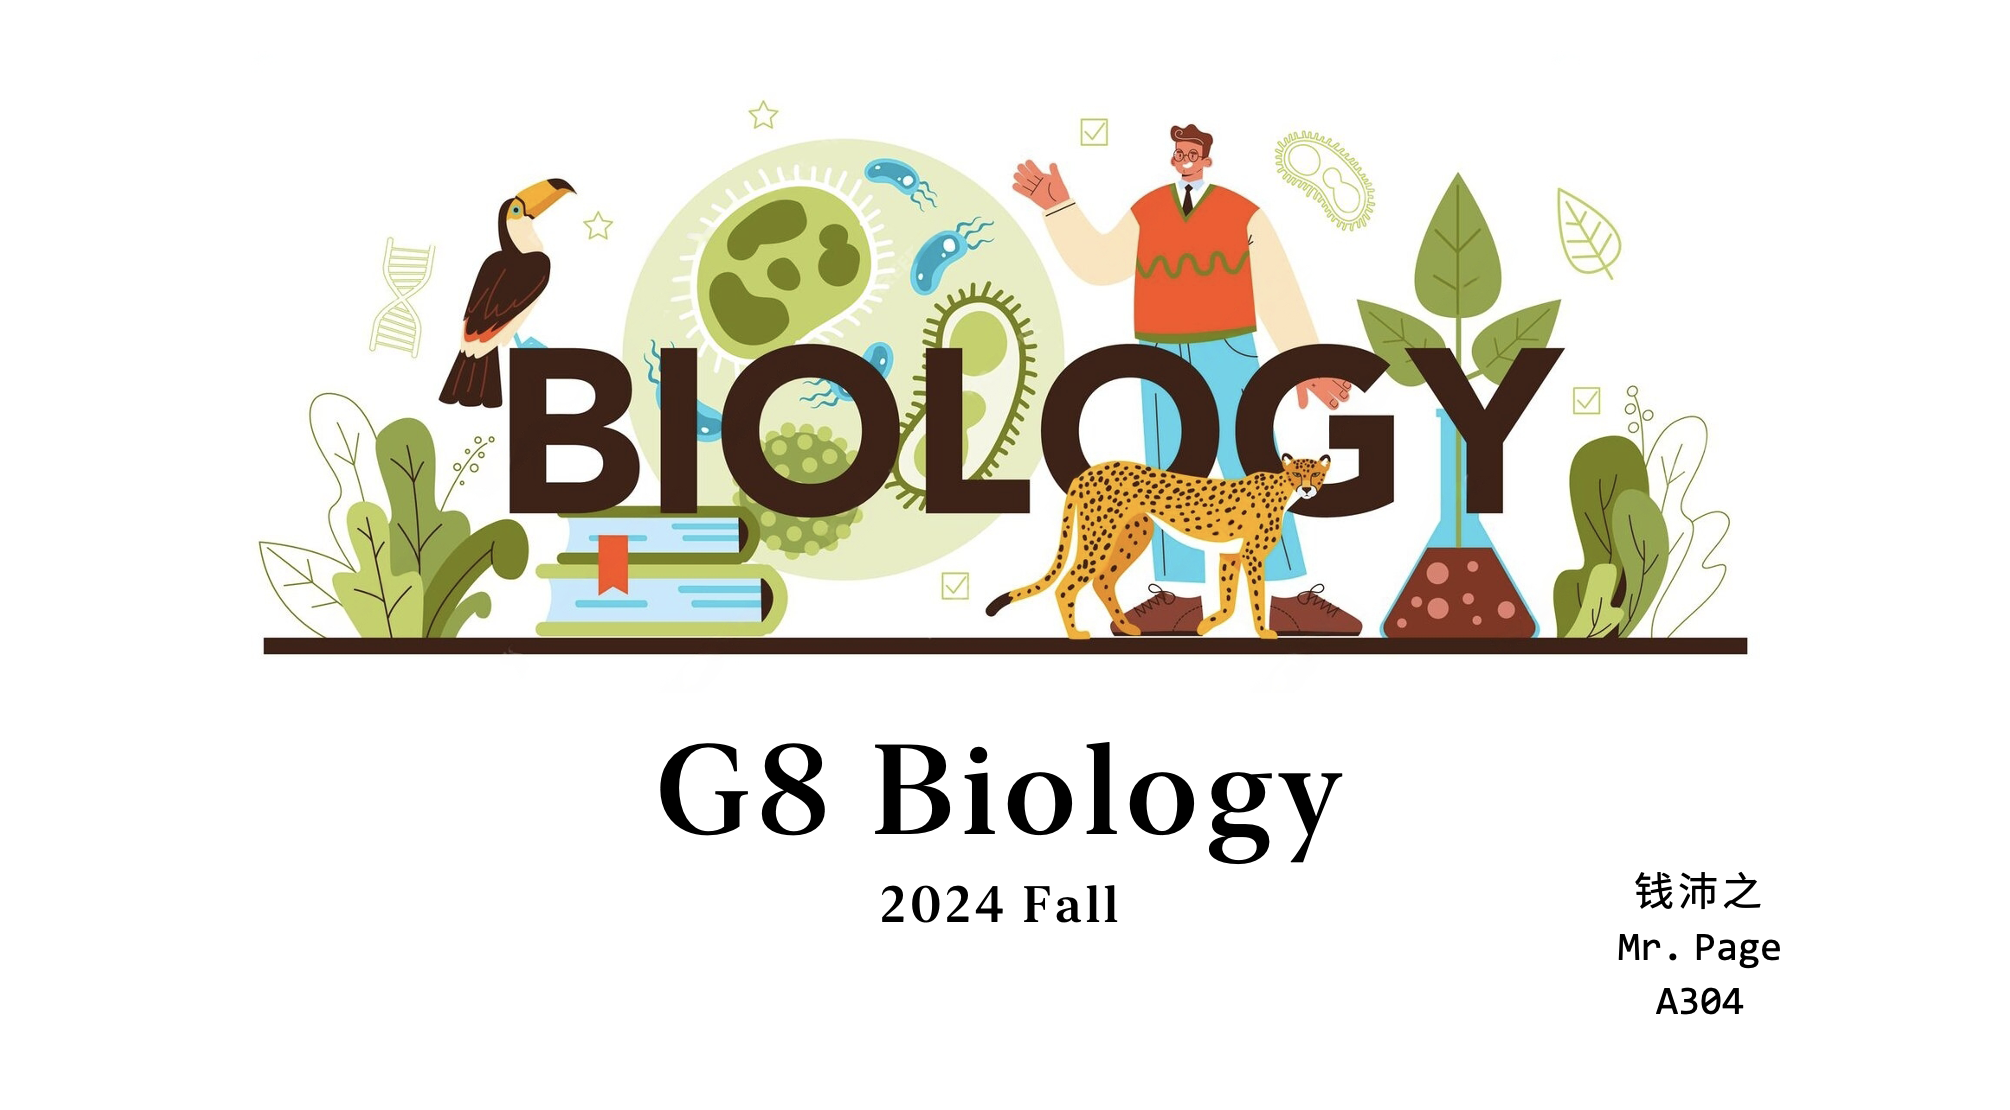
\includegraphics{./img/g8-bio.png}

\hypertarget{chapter-i-from-a-cell-to-an-organism}{%
\chapter{Chapter I: From A Cell To An Organism}\label{chapter-i-from-a-cell-to-an-organism}}

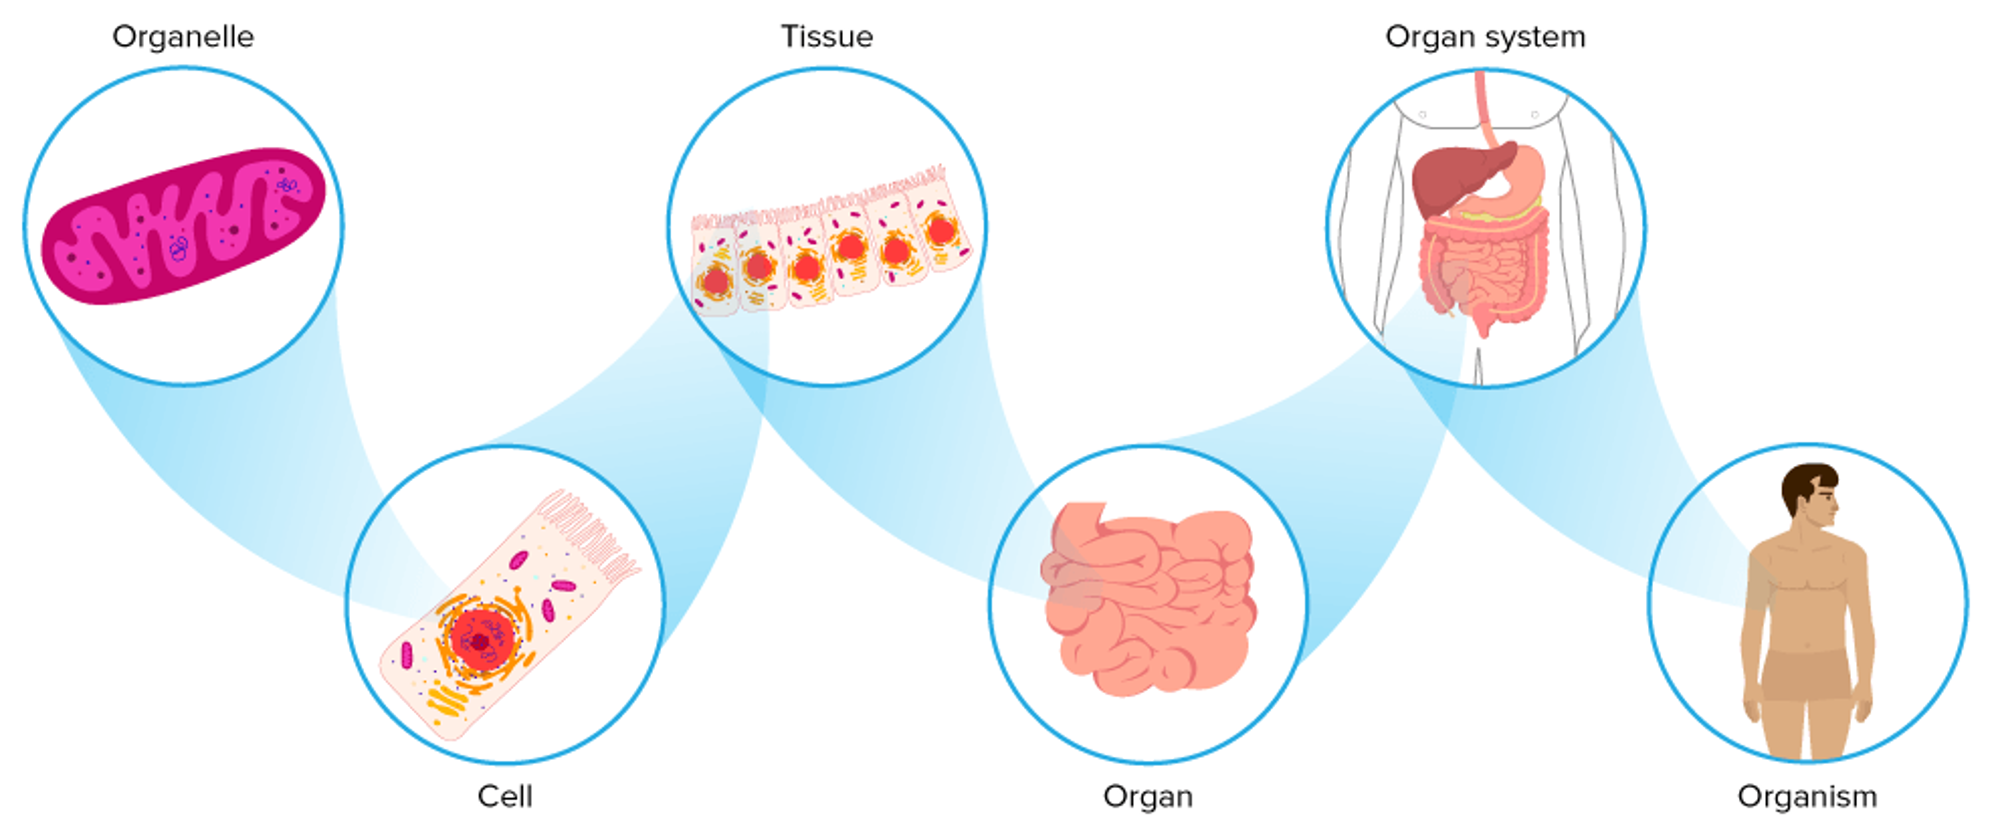
\includegraphics{./img/ch1.png}

\hypertarget{lecture-1-cell-cycle}{%
\section{Lecture 1: Cell Cycle}\label{lecture-1-cell-cycle}}

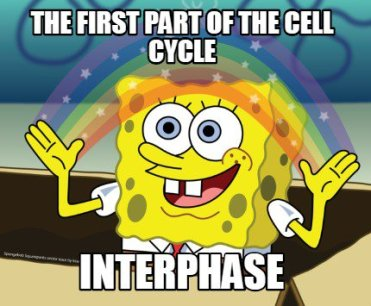
\includegraphics{./img/l1.jpg}

\hypertarget{lecture-2-cell-division}{%
\section{Lecture 2: Cell Division}\label{lecture-2-cell-division}}

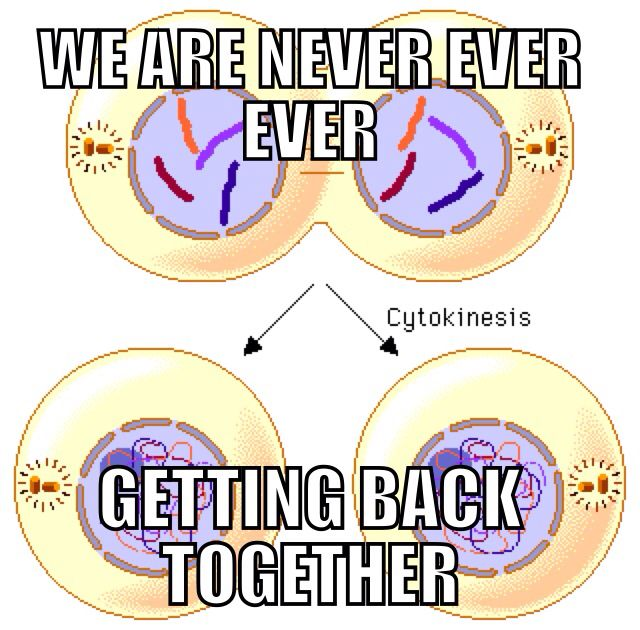
\includegraphics{./img/l2.jpg}

\hypertarget{lecture-3-levels-of-organization}{%
\section{Lecture 3: Levels of Organization}\label{lecture-3-levels-of-organization}}

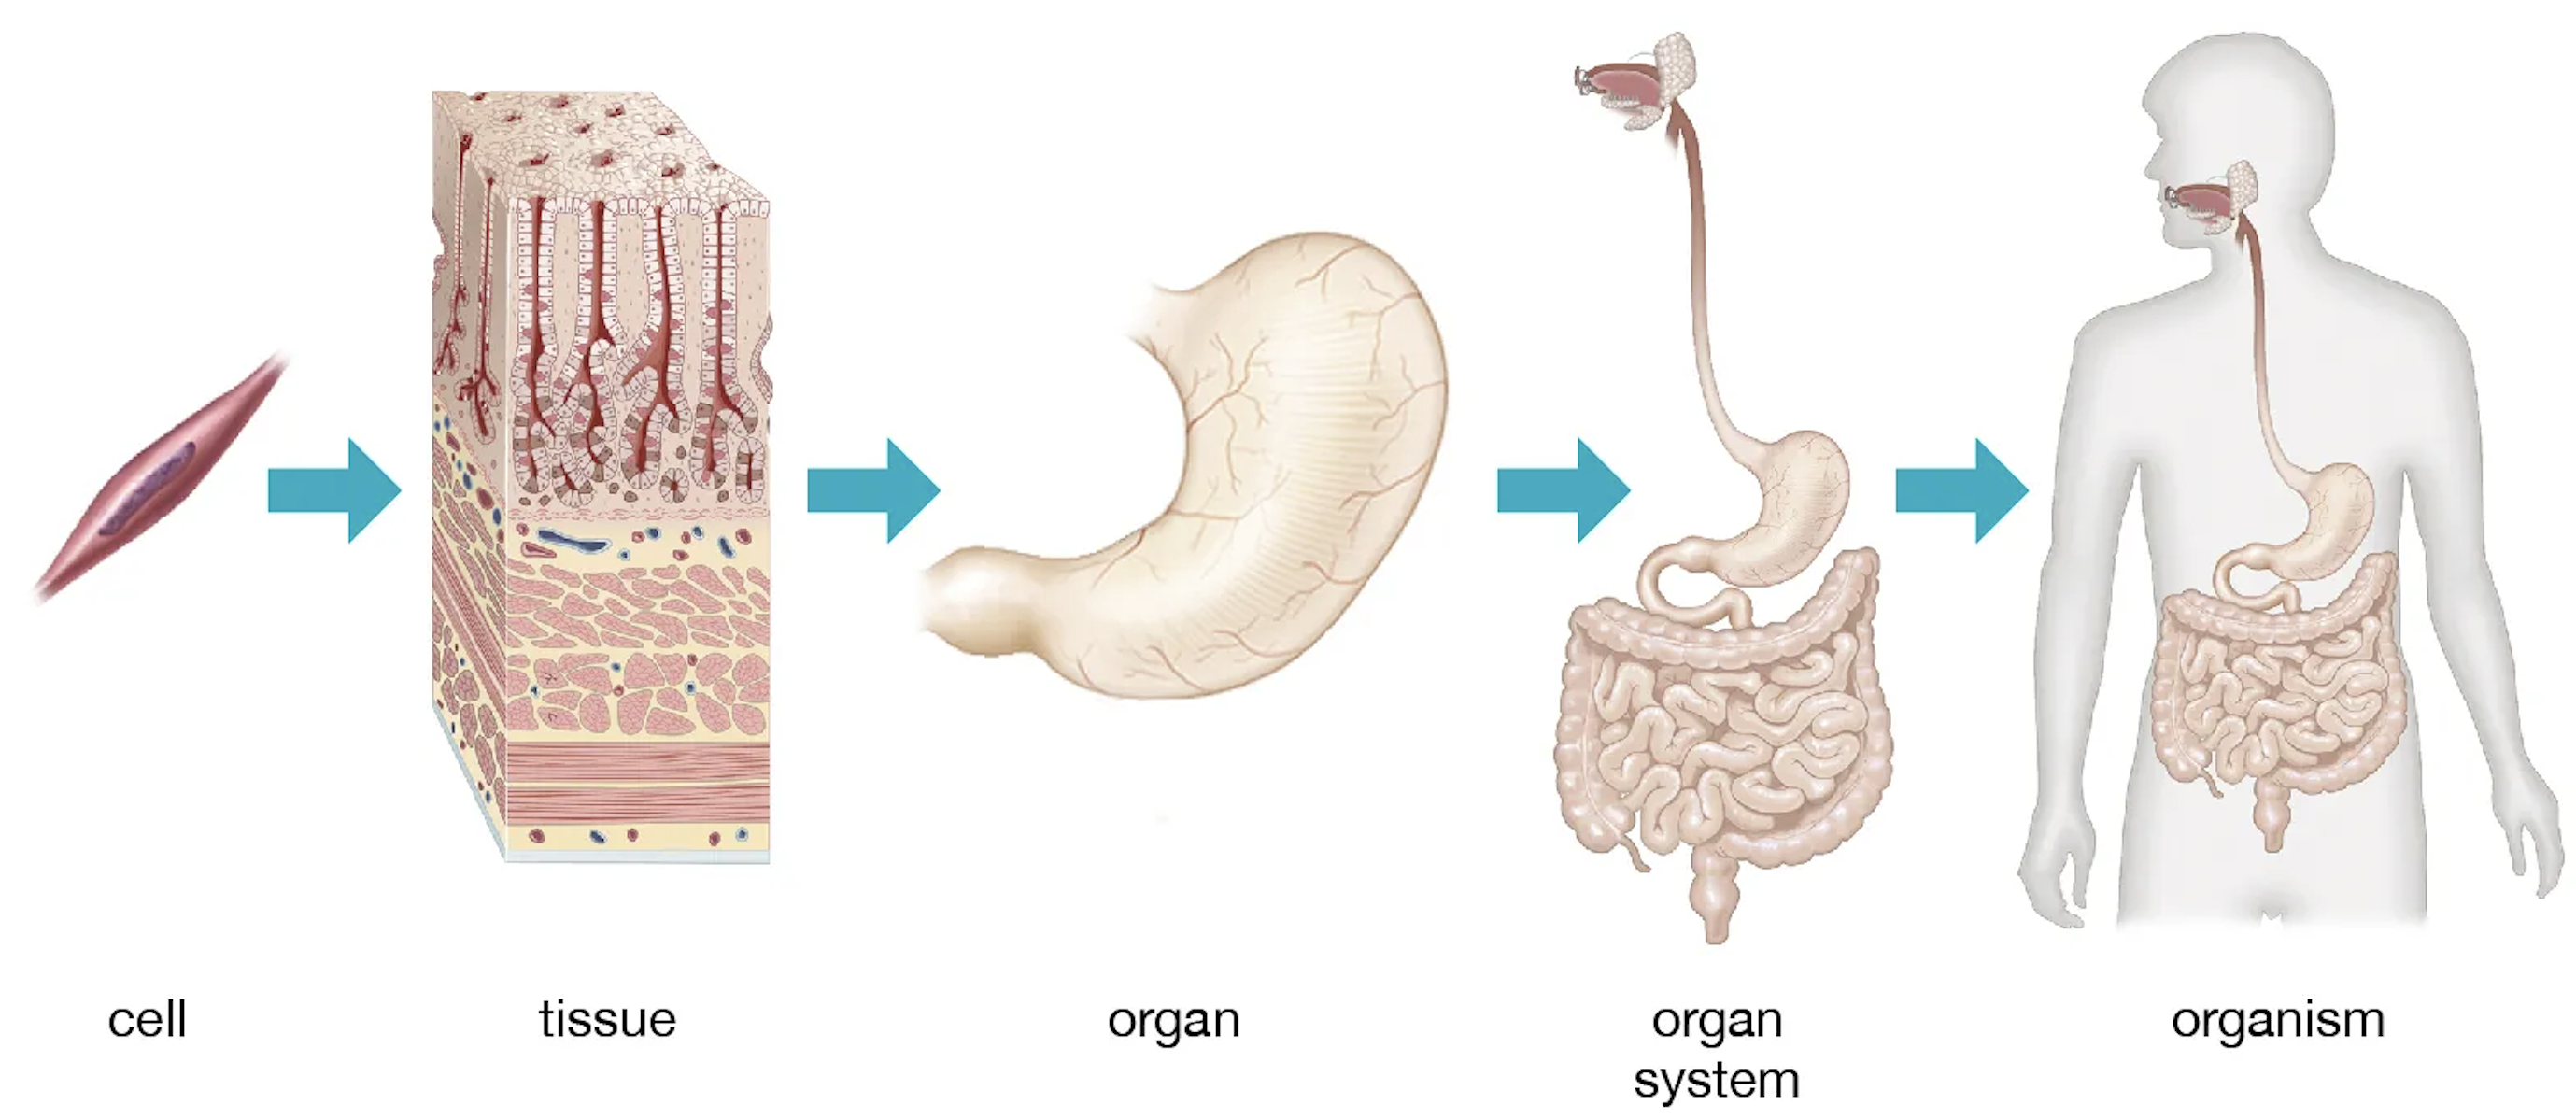
\includegraphics{./img/l3.png}

\hypertarget{experiment-1-observing-mitosis-in-plant-cells}{%
\section{Experiment 1: Observing Mitosis In Plant Cells}\label{experiment-1-observing-mitosis-in-plant-cells}}

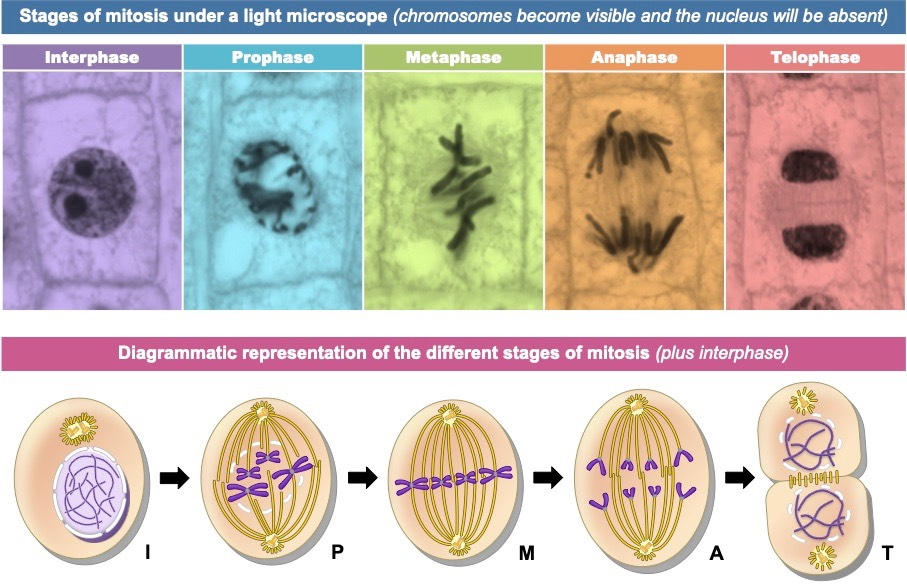
\includegraphics{./img/exp-1.jpeg}

\hypertarget{experiment-2-cell-differentiation}{%
\section{Experiment 2: Cell Differentiation}\label{experiment-2-cell-differentiation}}

\includegraphics{./img/exp-2-1.jpg}

\includegraphics{./img/exp-2-2.jpg}

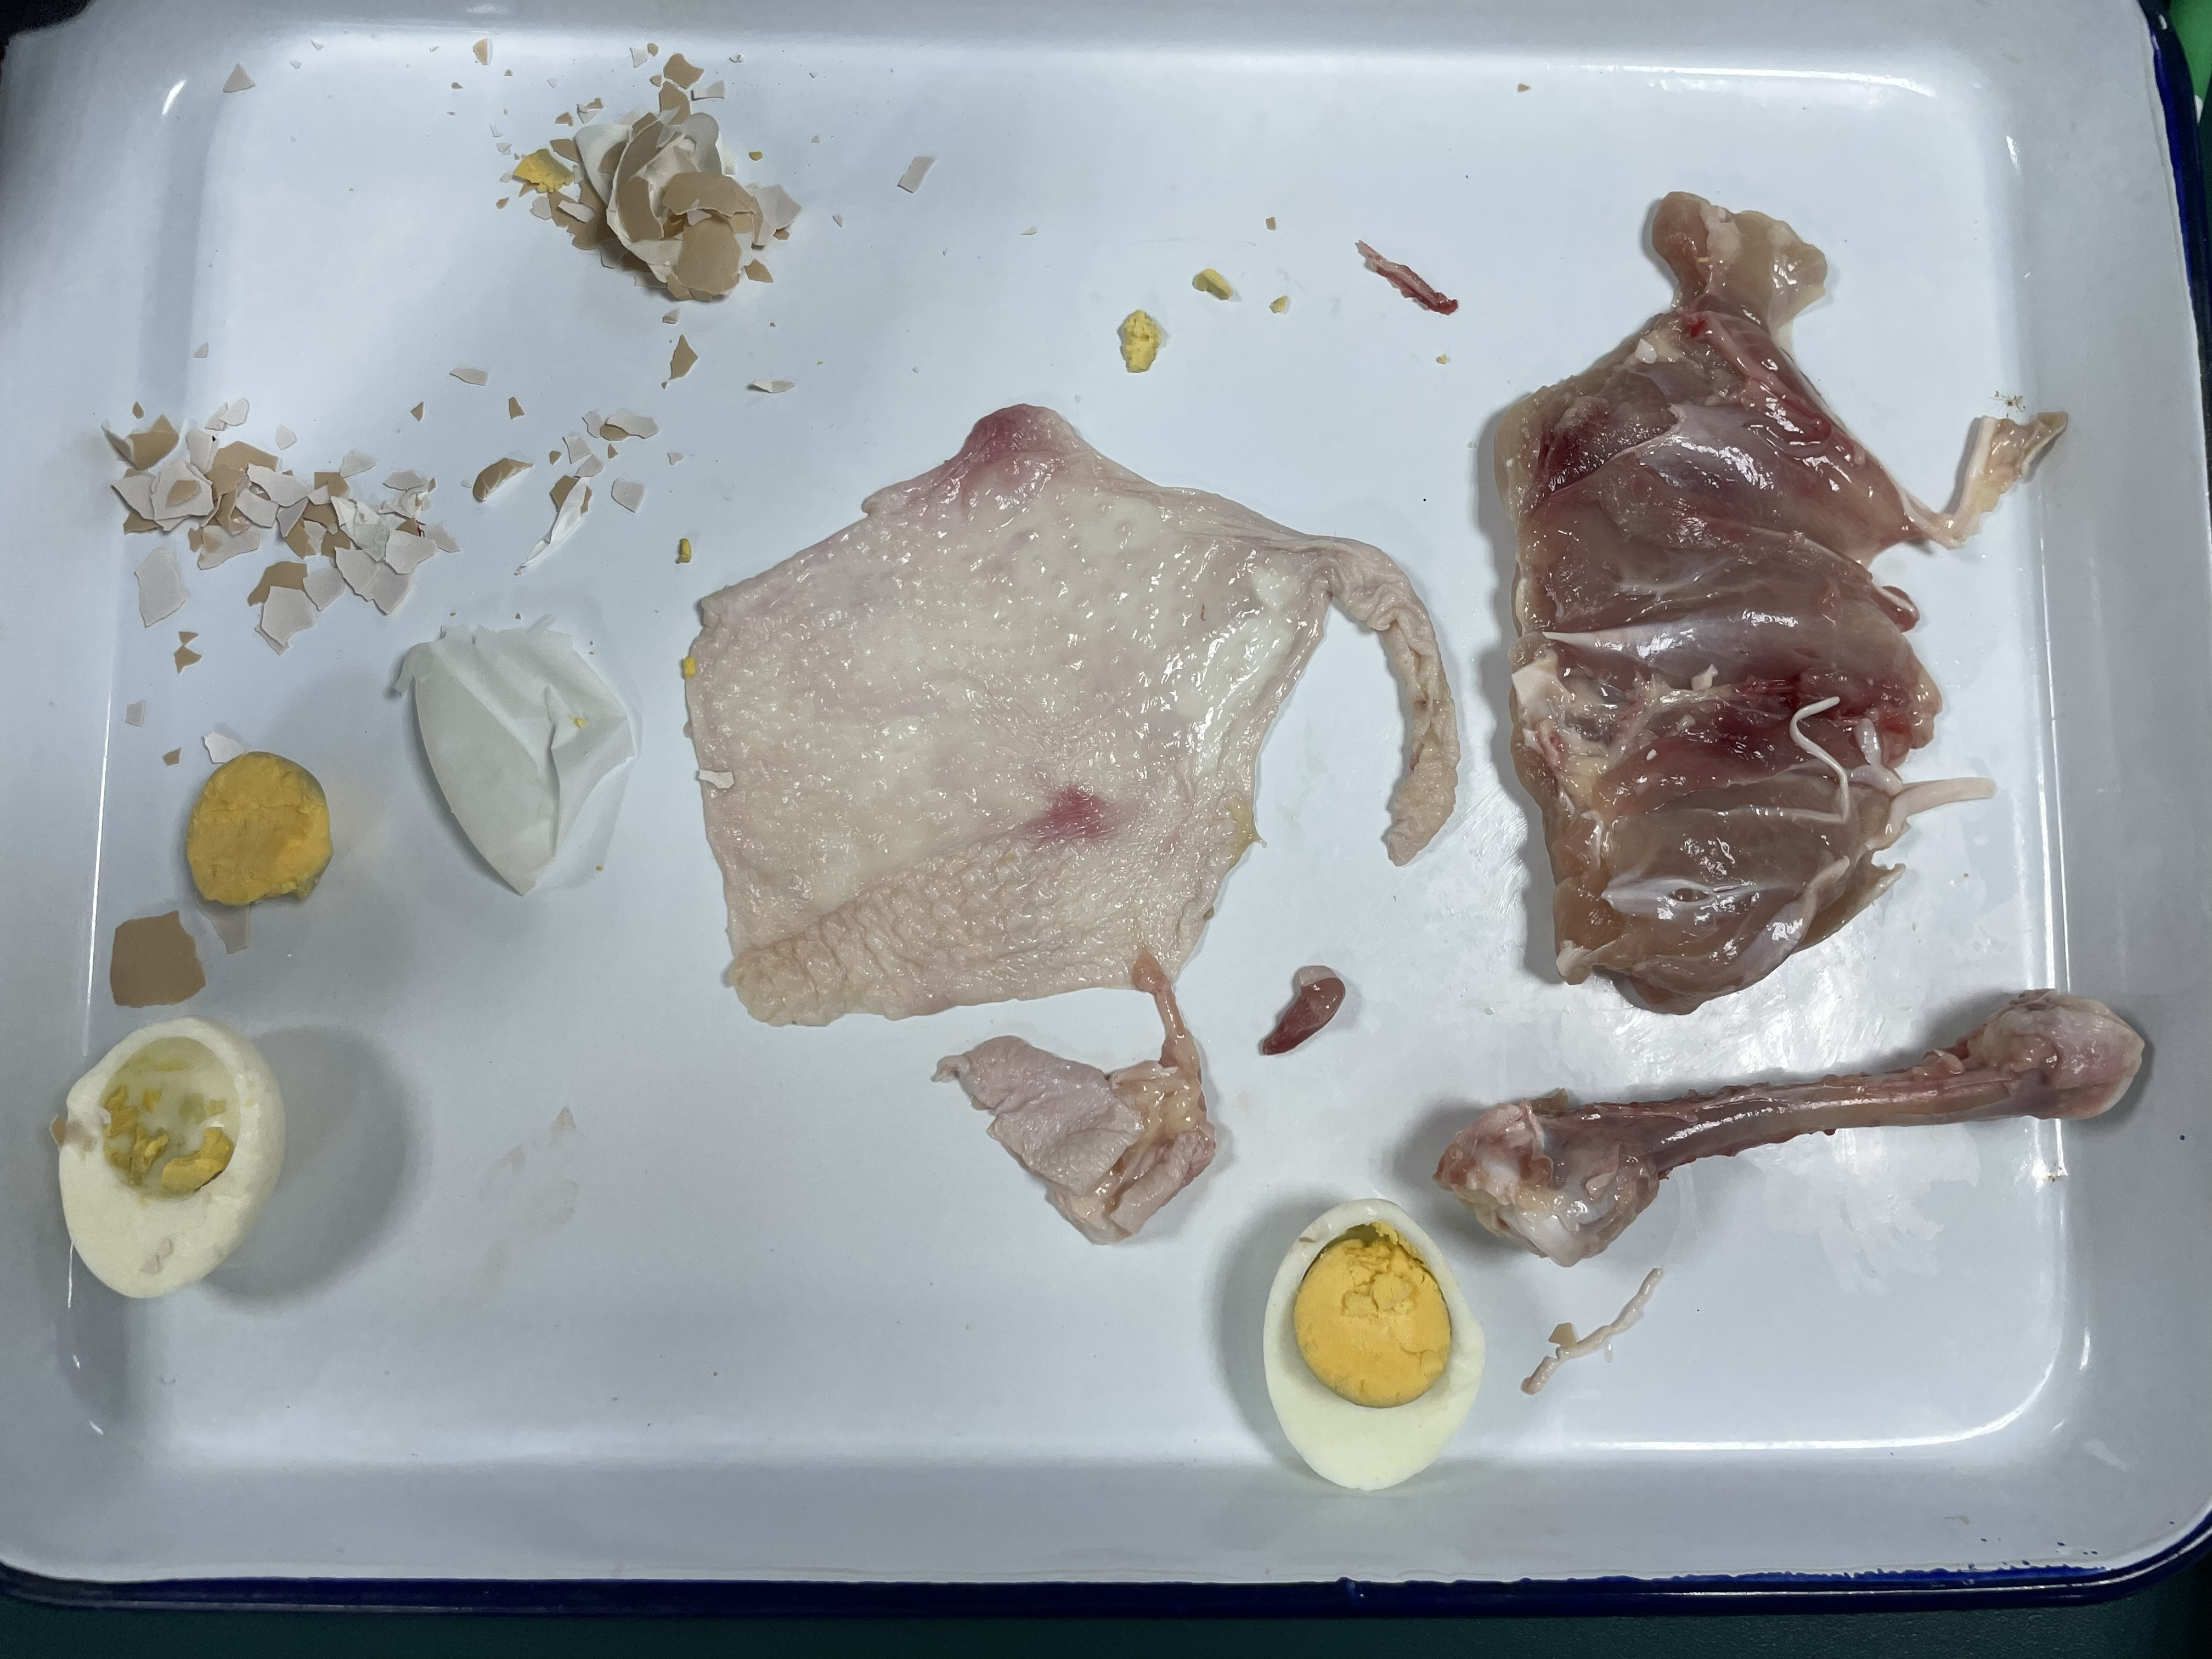
\includegraphics{./img/exp-2-3.jpg}

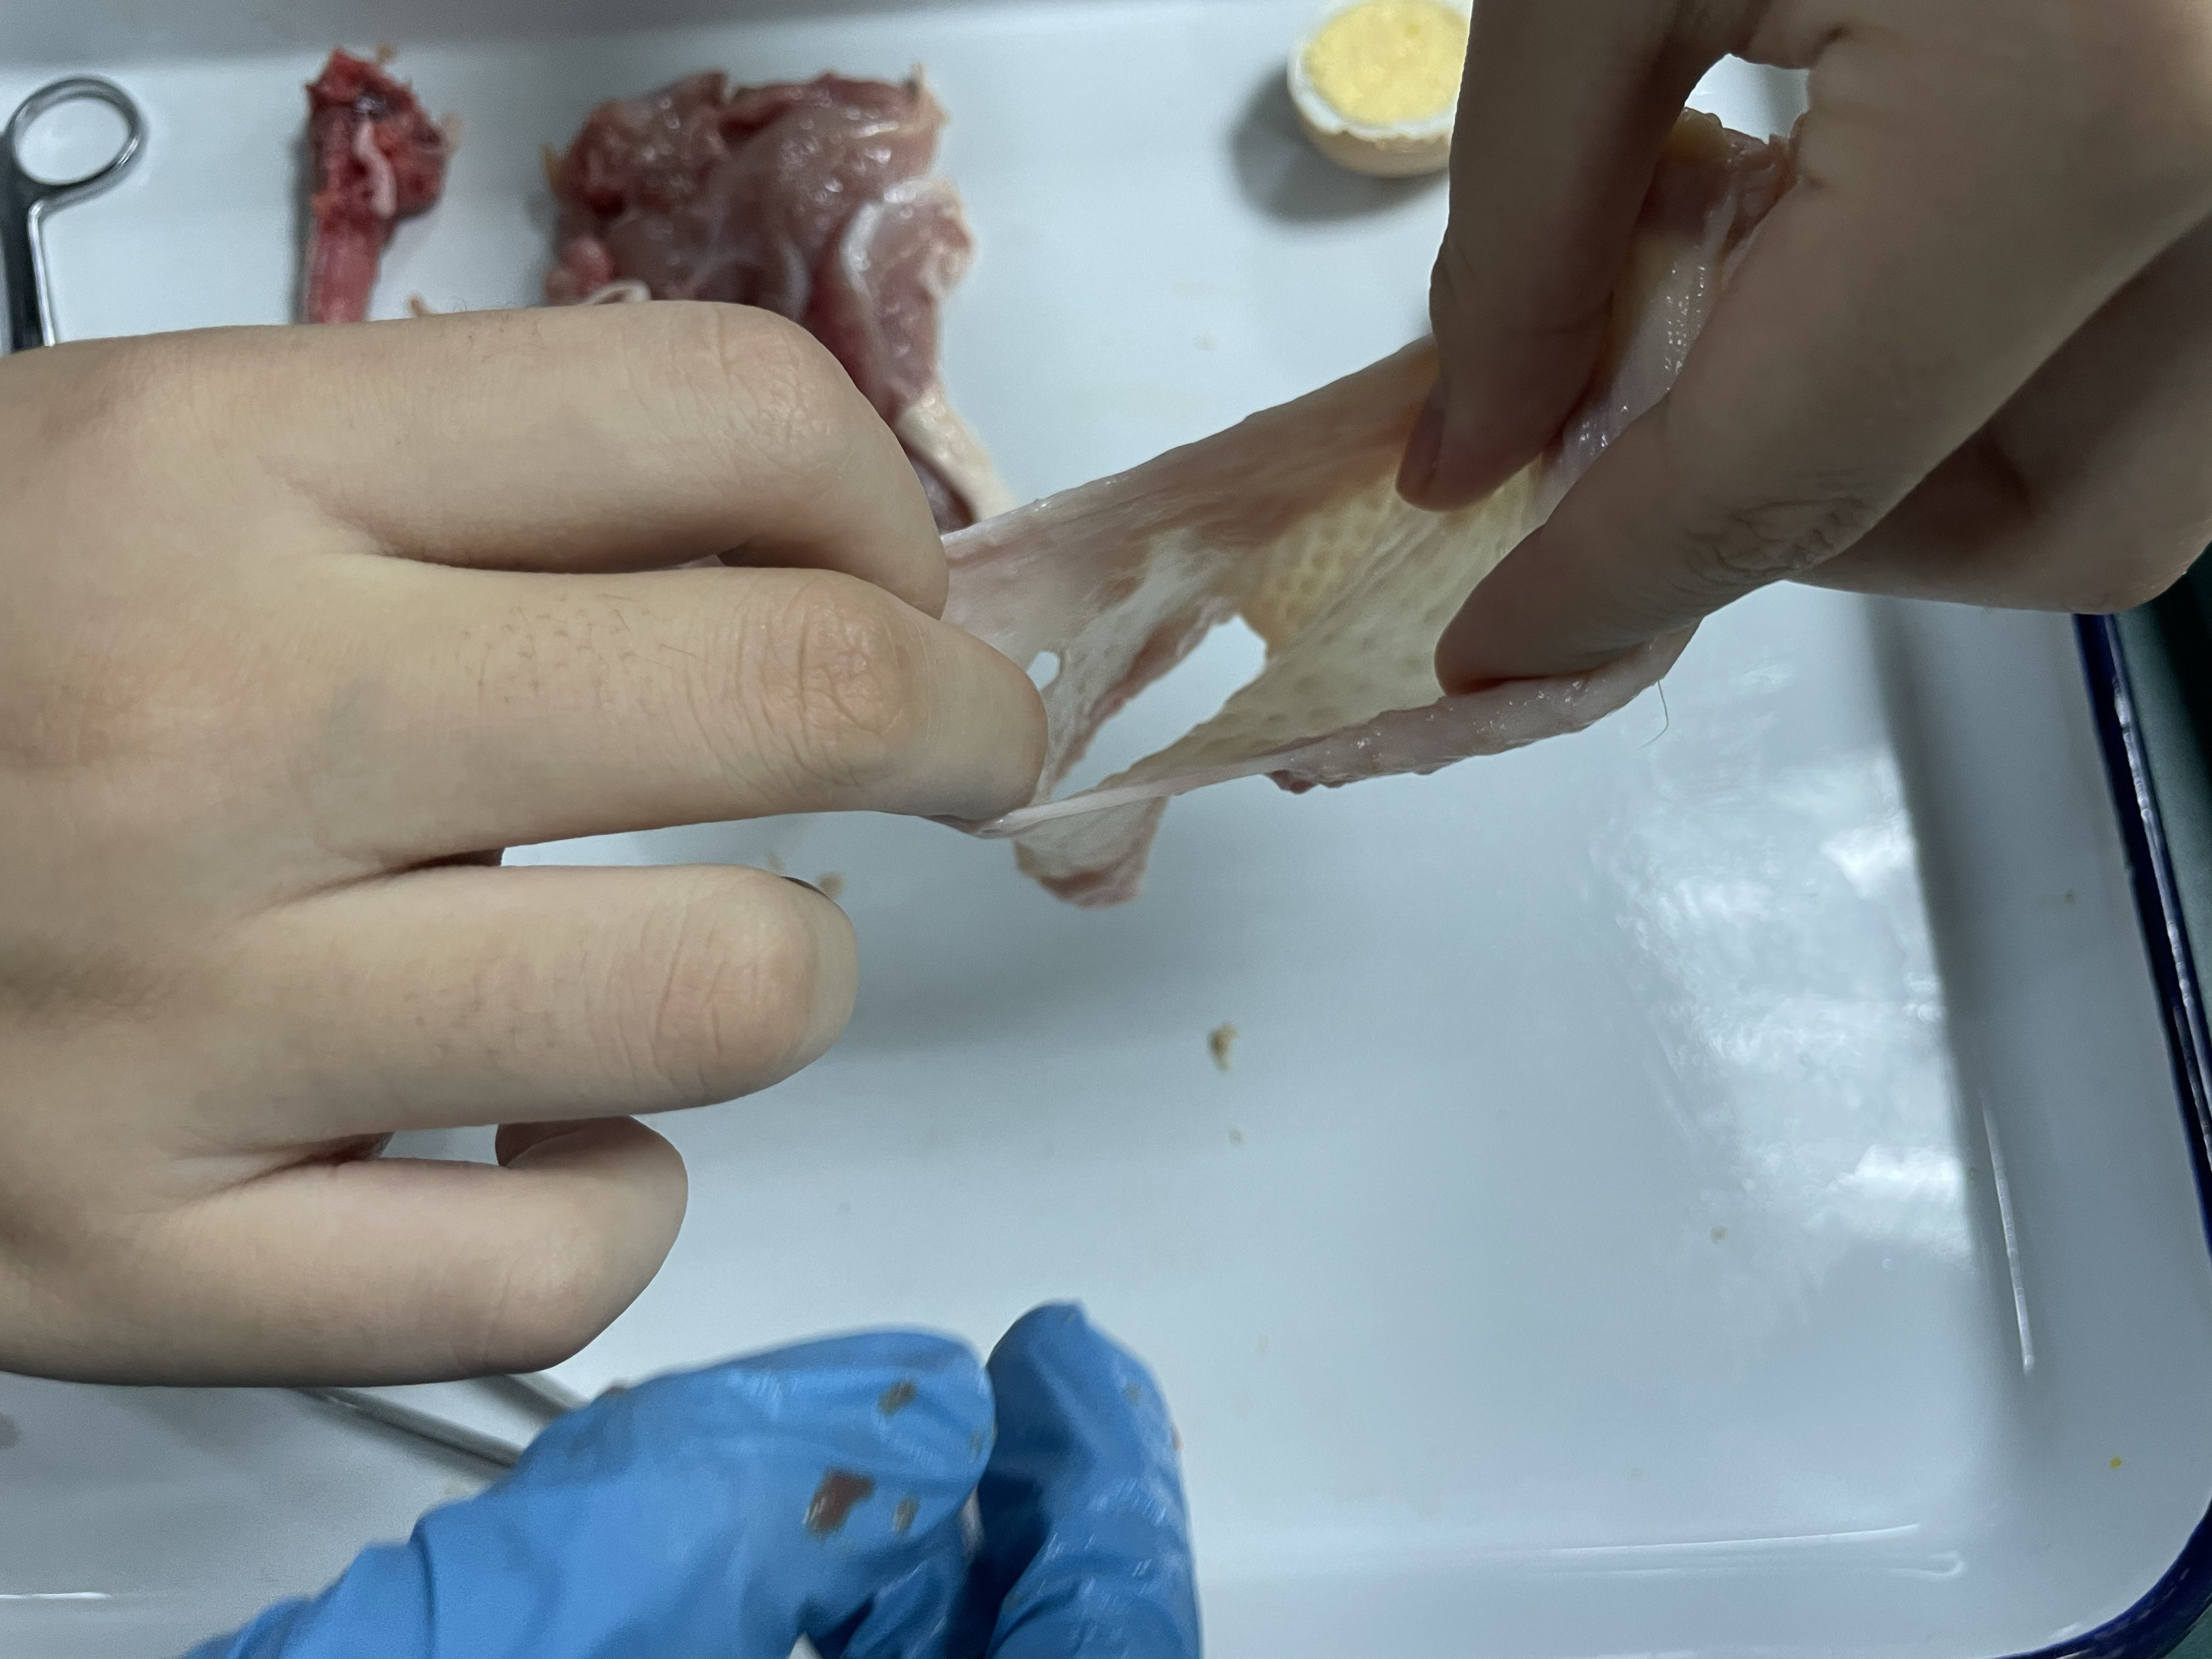
\includegraphics{./img/exp-2-4.jpg}

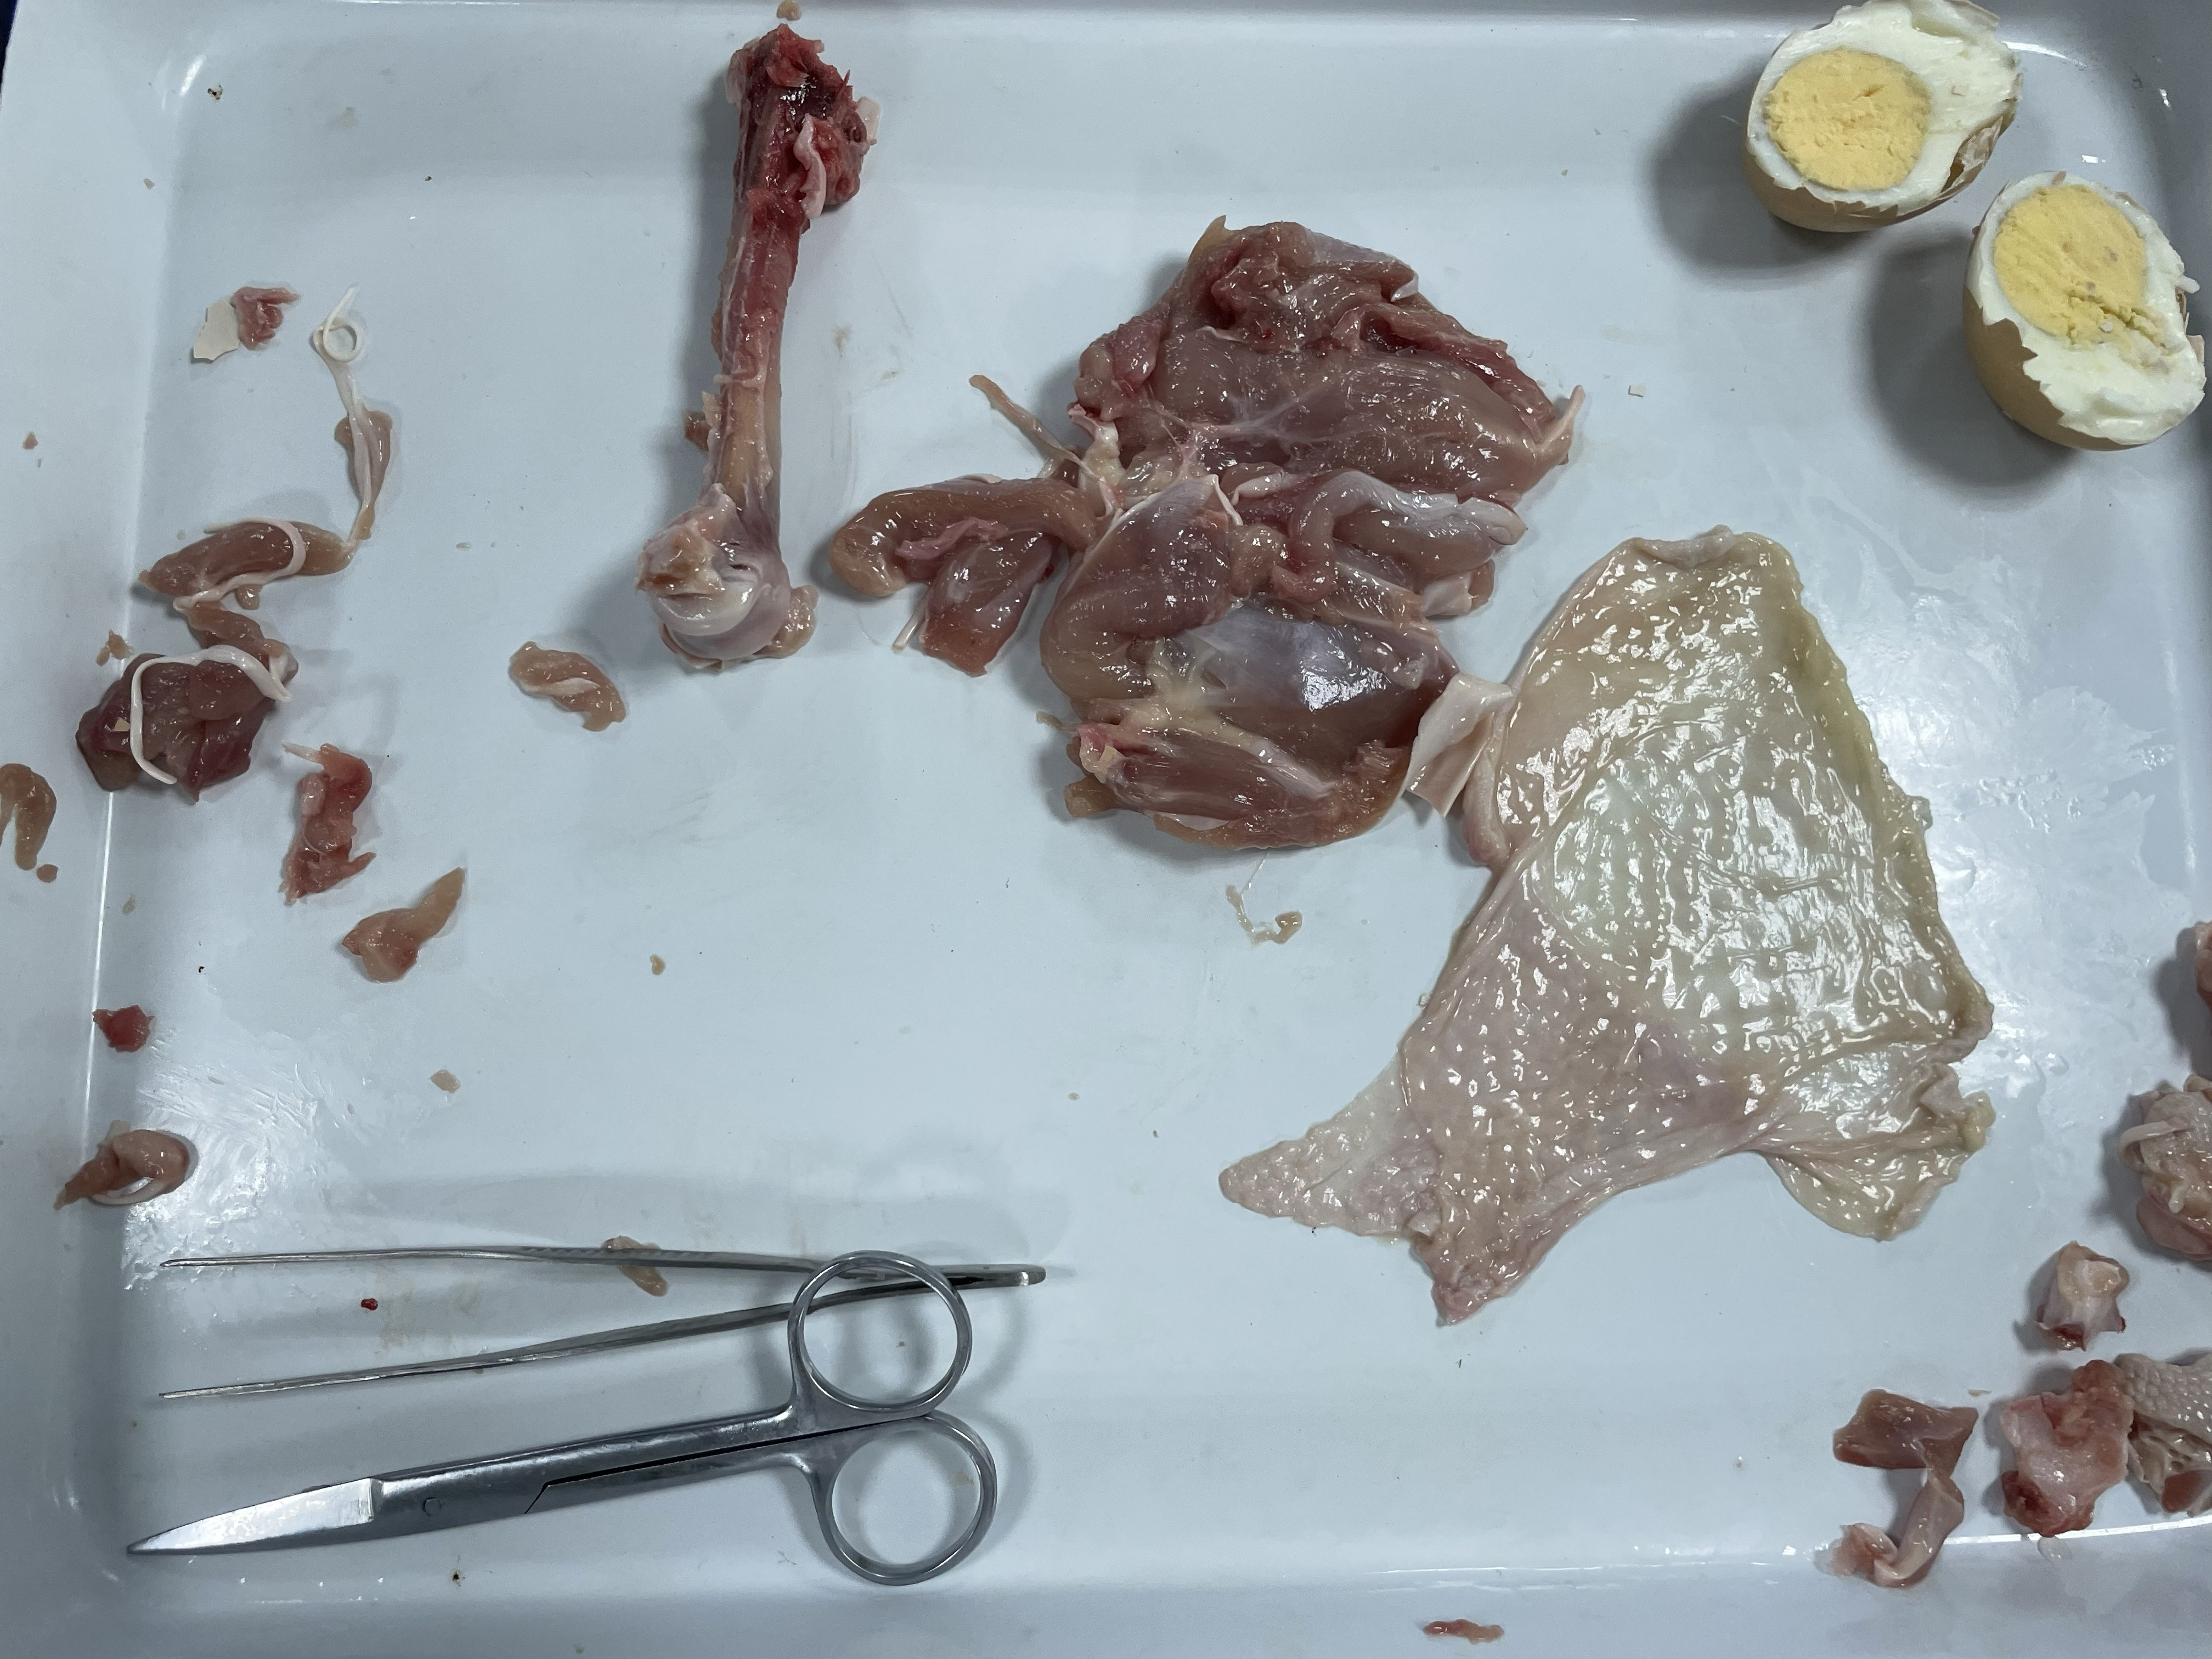
\includegraphics{./img/exp-2-5.jpg}

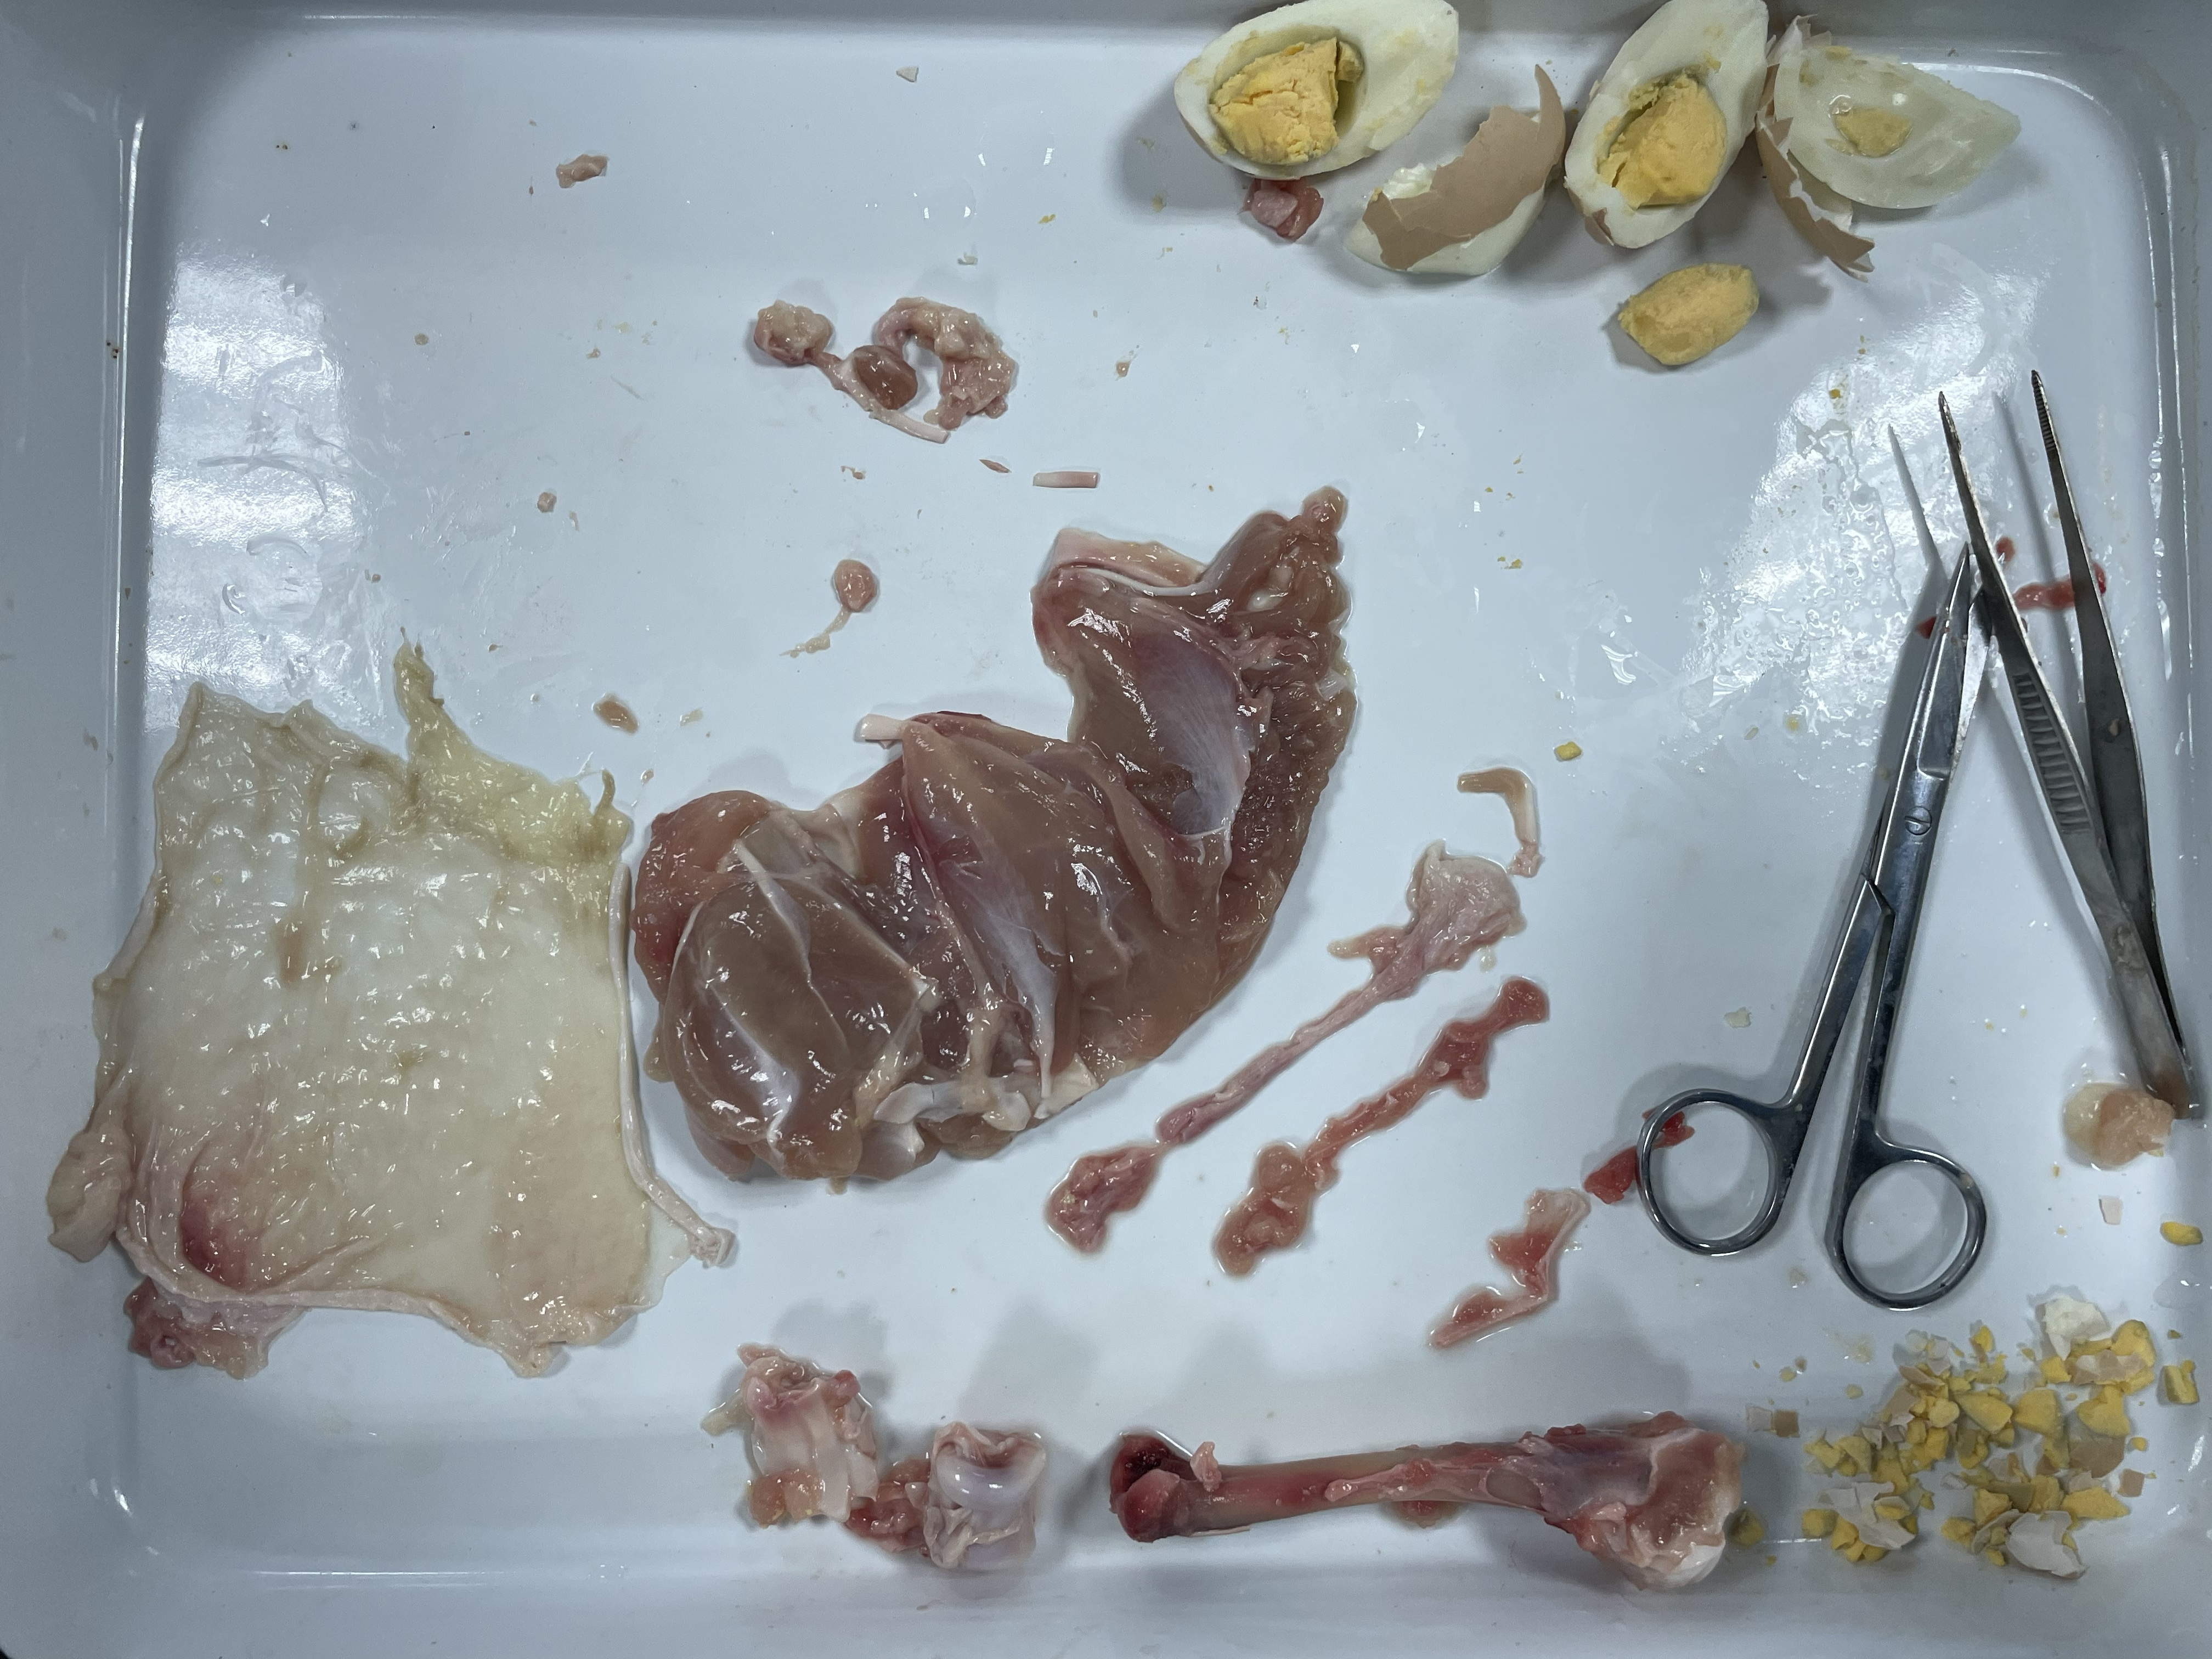
\includegraphics{./img/exp-2-6.jpg}

\hypertarget{project-1-mitosis-the-cell-cycle}{%
\section{Project 1: Mitosis \& The Cell Cycle}\label{project-1-mitosis-the-cell-cycle}}

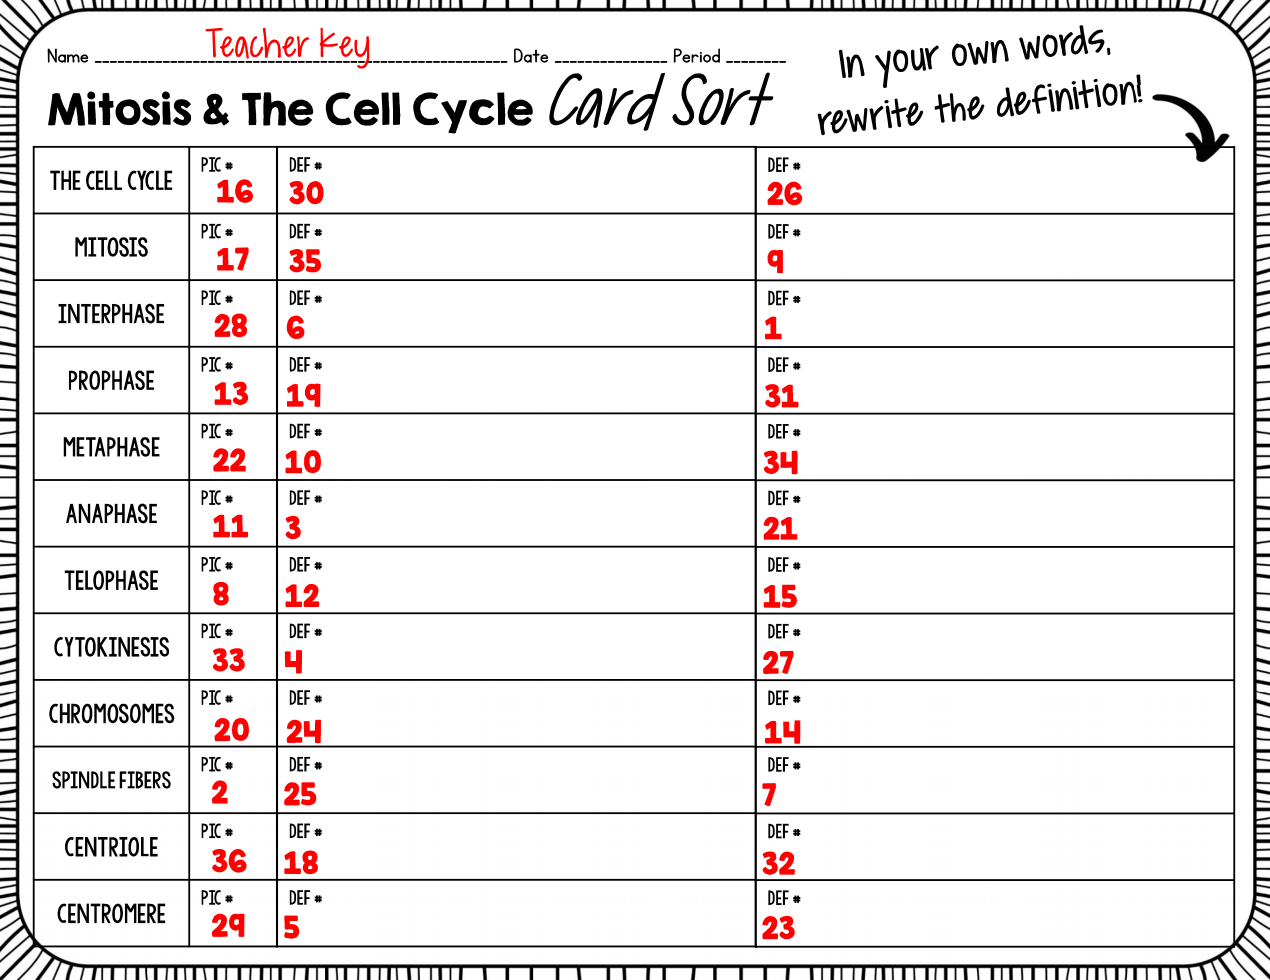
\includegraphics{./img/p1-1.png}

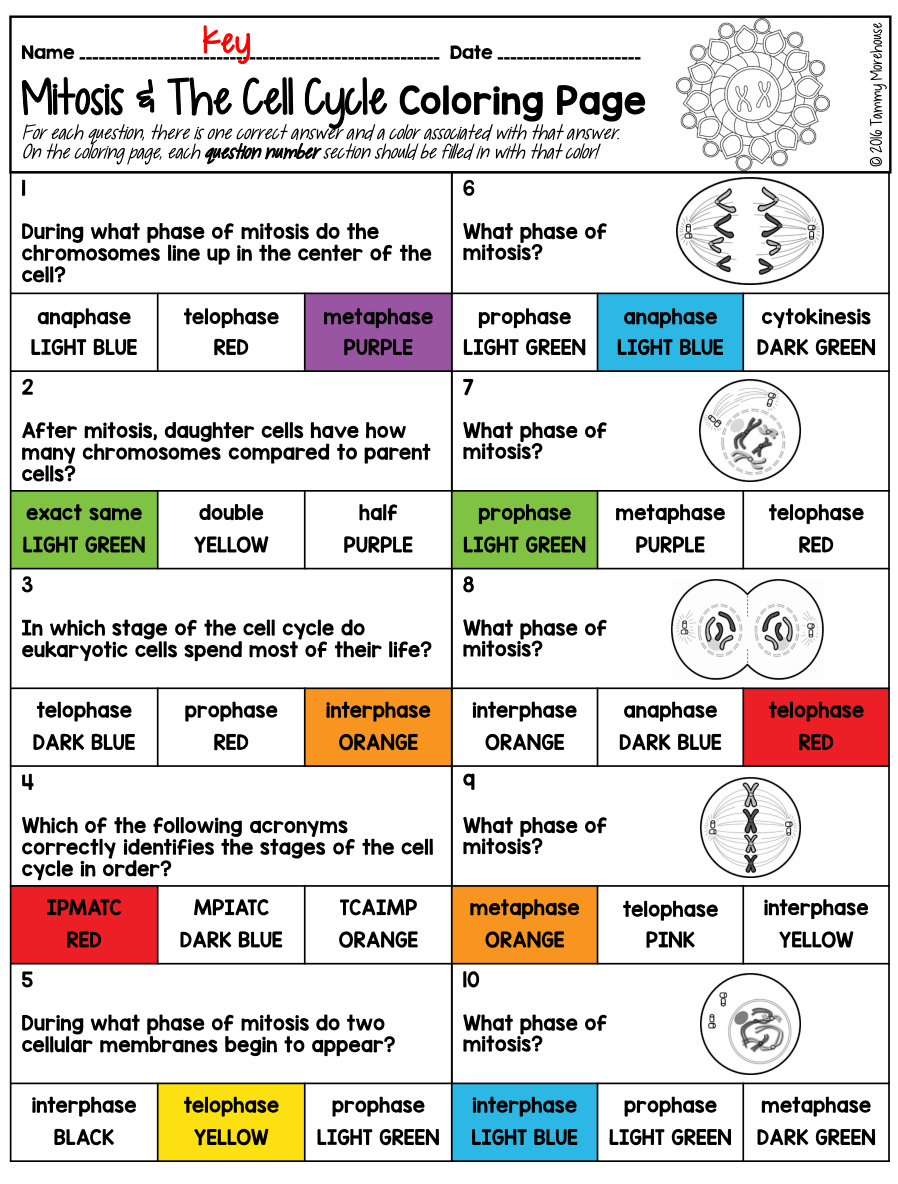
\includegraphics{./img/p1-2.png}

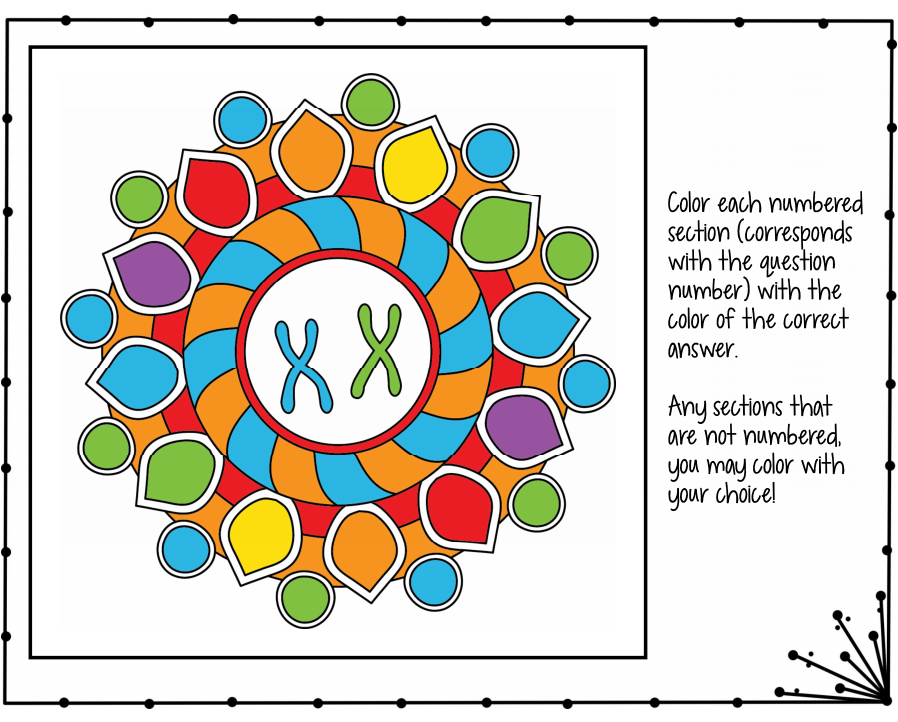
\includegraphics{./img/p1-3.png}

\hypertarget{project-2-biological-organization}{%
\section{Project 2: Biological Organization}\label{project-2-biological-organization}}

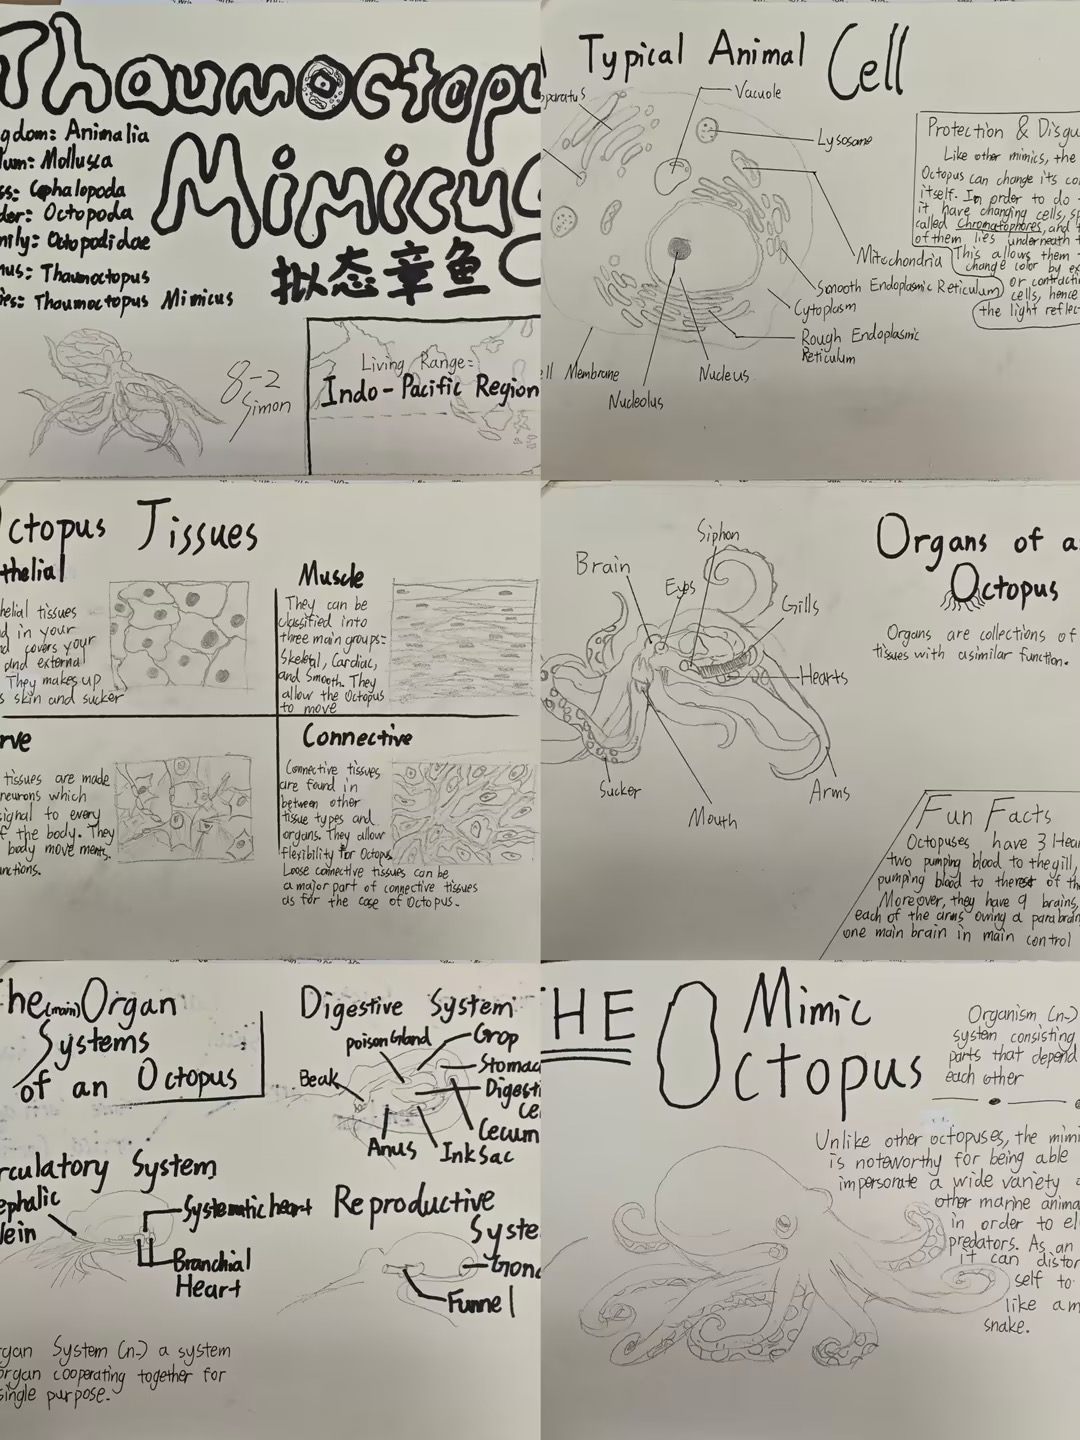
\includegraphics{./img/p2-1.jpg}

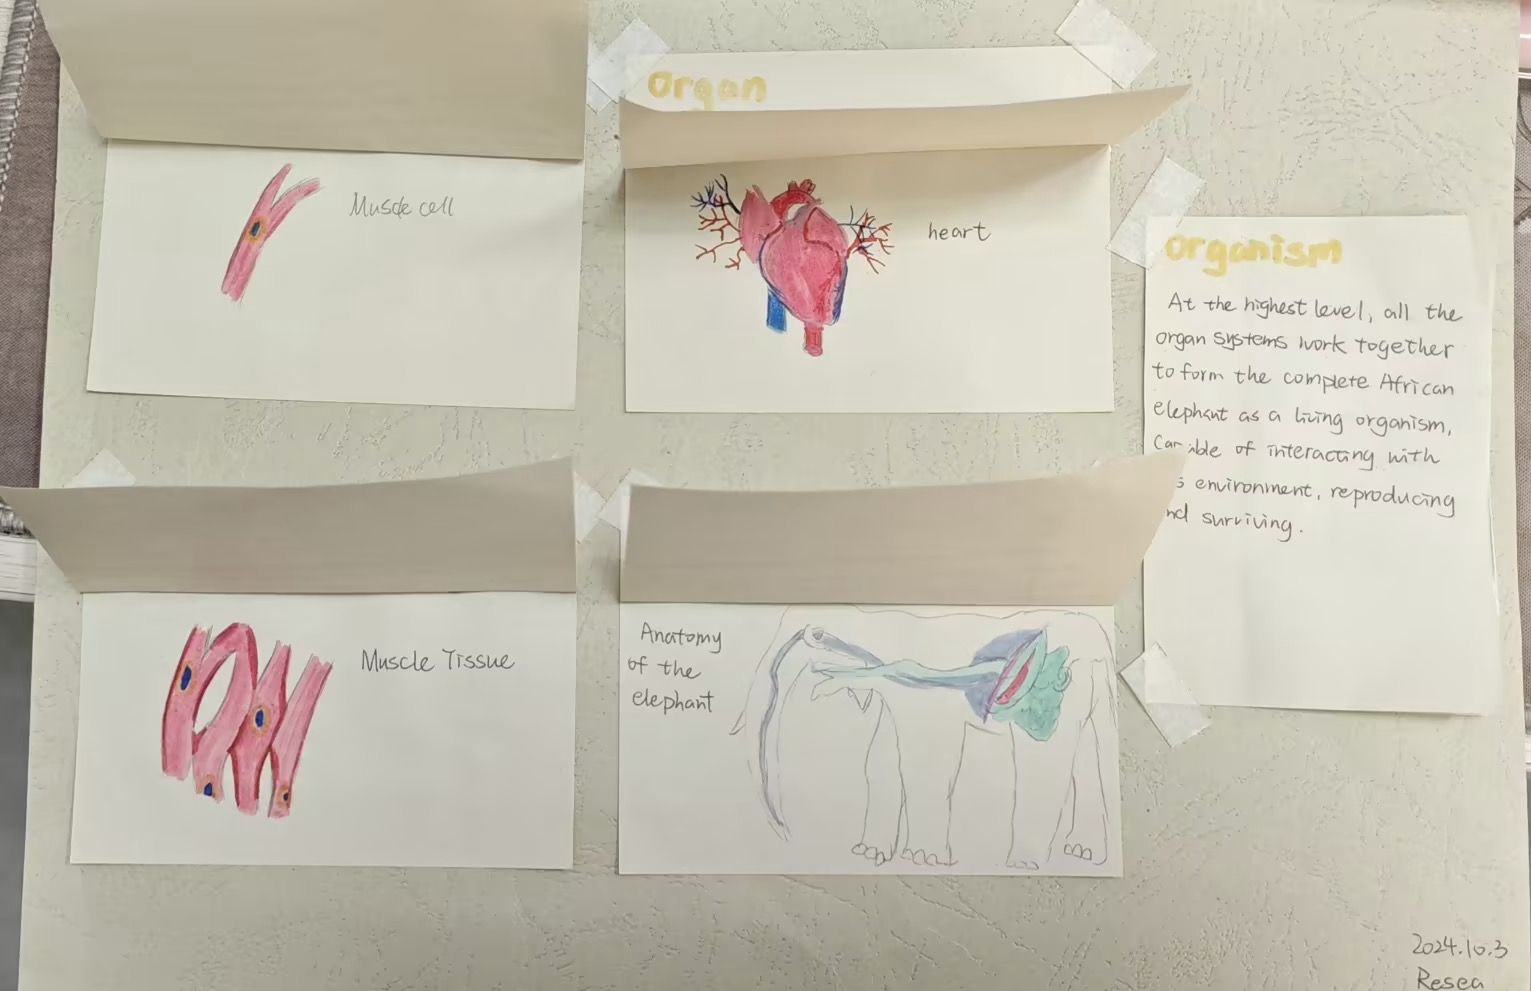
\includegraphics{./img/p2-2.jpg}

\hypertarget{chapter-ii-reproduction-of-organisms}{%
\chapter{Chapter II: Reproduction Of Organisms}\label{chapter-ii-reproduction-of-organisms}}

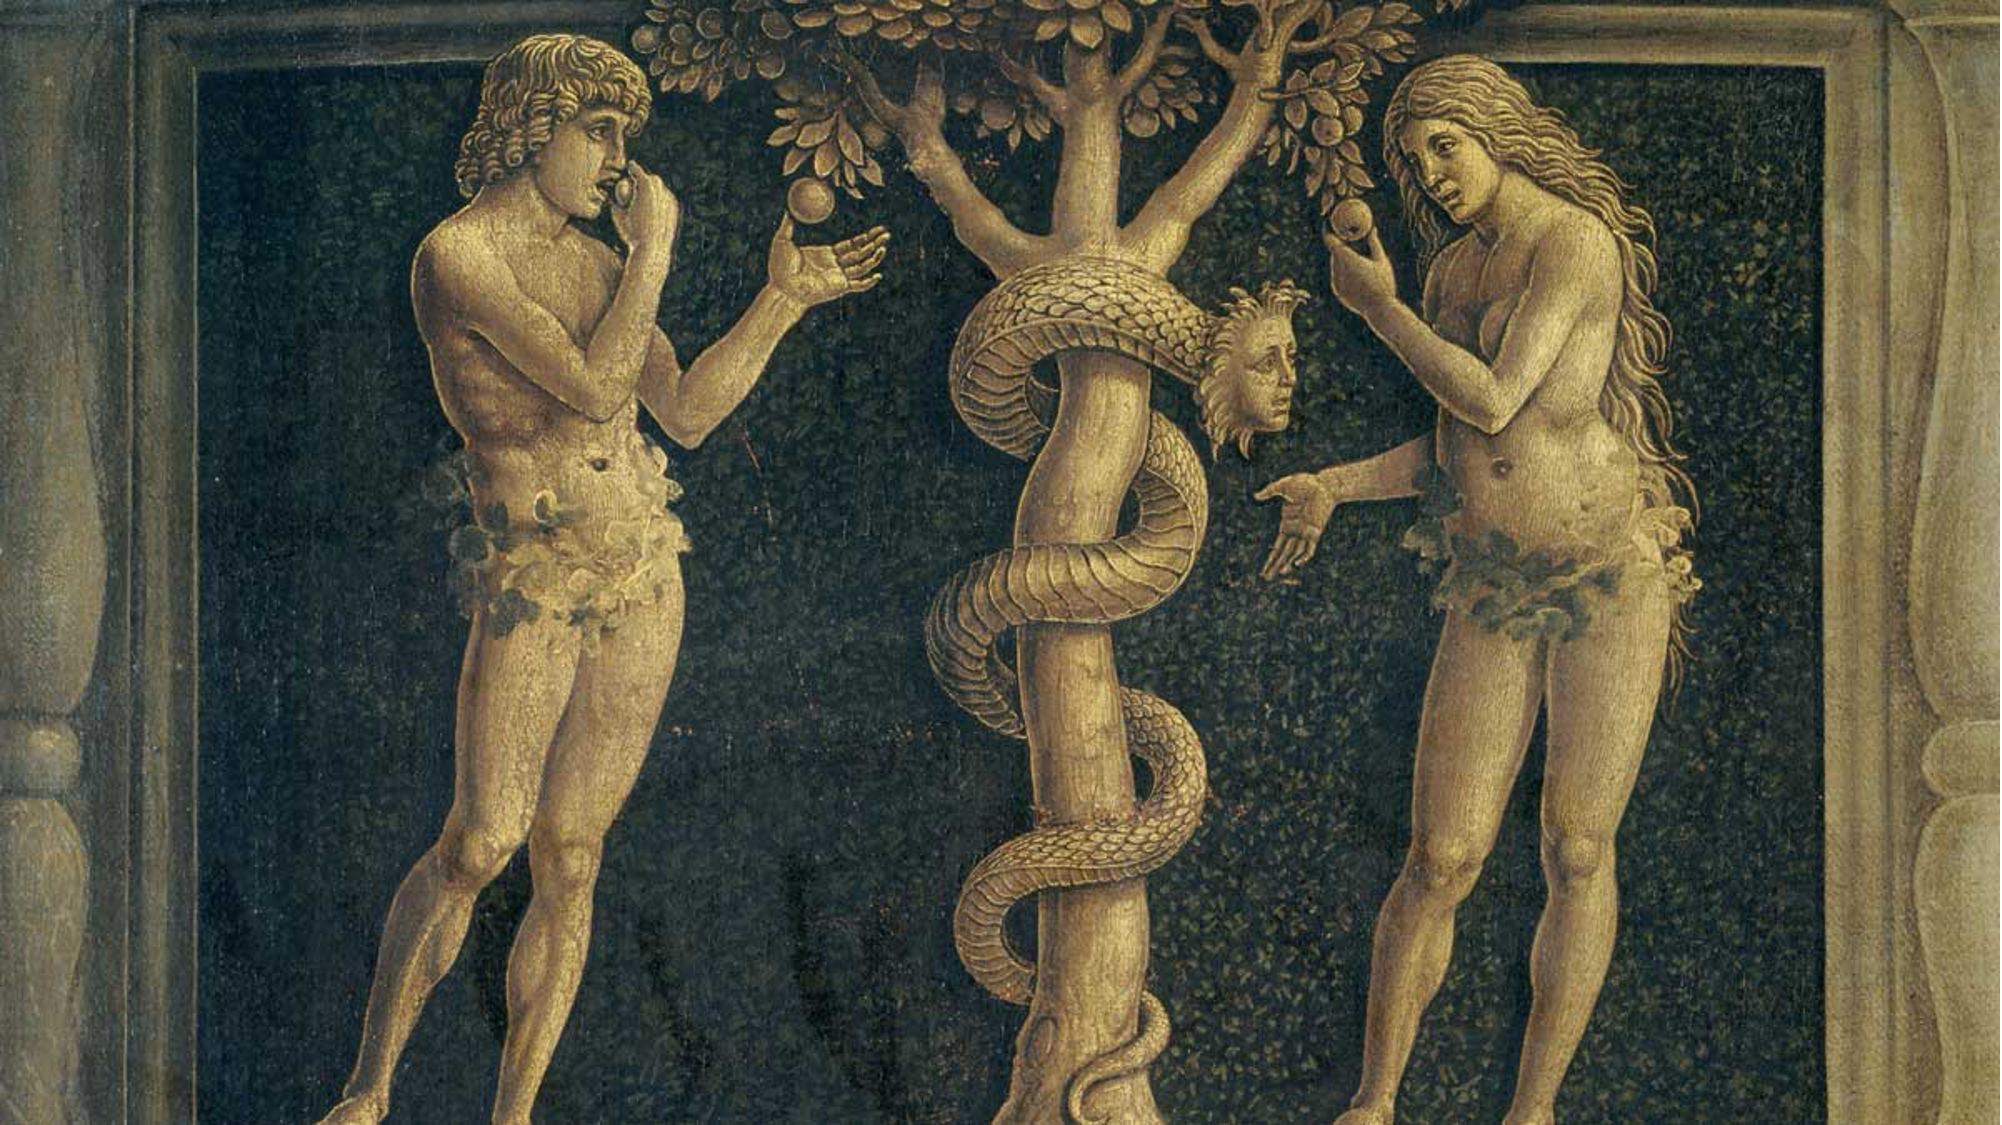
\includegraphics{./img/ch2.png}

\hypertarget{lecture-4-sexual-reproduction}{%
\section{Lecture 4: Sexual Reproduction}\label{lecture-4-sexual-reproduction}}

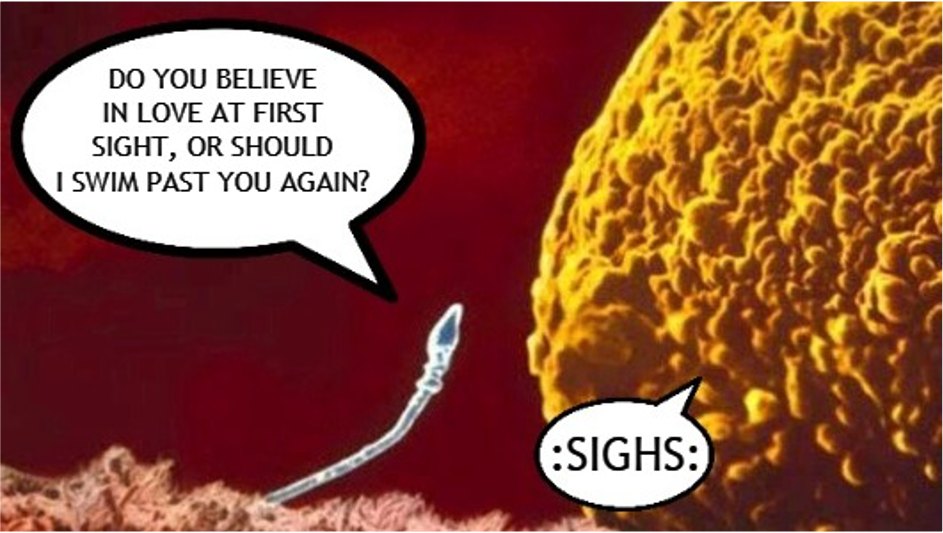
\includegraphics{./img/sperm-egg-meme.png}

\hypertarget{keywords}{%
\subsection{Keywords}\label{keywords}}

\begin{longtable}[]{@{}cc@{}}
\toprule\noalign{}
英文 & 中文 \\
\midrule\noalign{}
\endhead
\bottomrule\noalign{}
\endlastfoot
Sexual Reproduction & 有性生殖 \\
Meiosis & 减数分裂 \\
Sperm & 精子 \\
Egg & 卵子 \\
Fertilization & 受精 \\
Zygote & 受精卵 \\
Haploid & 单倍体 \\
Diploid & 二倍体 \\
Homologous chromosomes & 同源染色体 \\
\end{longtable}

\hypertarget{lesson-outline}{%
\subsection{Lesson outline}\label{lesson-outline}}

\textbf{A. What is sexual reproduction?}\\
1. {Sexual reproduction} produces an offspring when genetic materials from two
different sex cells combine.\\
a. The female sex cell, a(n) {egg}, forms in an ovary.\\
b. The male sex cell, a(n) {sperm}, forms in a testis.\\
2. During a process called {fertilization}, an egg cell and a sperm cell join together. The
new cell that forms is called a(n) {zygote}.

\textbf{B. Diploid Cells}\\
1. Organisms that reproduce sexually make two kinds of cells---{body} cells and sex cells.\\
2. Body cells are {diploid}; they have pairs of chromosomes.\\
3. If a zygote has too many or too few {chromosomes}, it will not develop properly.\\
4. Different organisms have different {numbers} of chromosomes.\\
5. {Homologous chromosomes} are pairs of chromosomes that have genes for the same traits arranged in the same order.

\textbf{C. Haploid Cells}\\
1. Sex cells are {haploid}; they have only one chromosome from each pair of chromosomes.\\
2. In {meiosis}, one diploid cell divides and makes four haploid cells.

\hypertarget{homework}{%
\subsection{Homework}\label{homework}}

\textbf{Matching}\\
1. G\\
2. B\\
3. H\\
4. C\\
5. I\\
6. A\\
7. D\\
8. F\\
9. E

\textbf{Multiple Choice Questions}\\
10. A\\
11. B

\textbf{Short Answer Questions}\\
12. Sexual reproduction is the {production of an offspring} that results when the genetic material from two different cells combine.\\
(Hint: Check ``how to write a definition'' in extension)\\
{s}\\
13. A zygote is {a new cell} that forms when an egg cell and a sperm cell join during fertilization.\\
(Hint: Check ``how to write a definition'' in extension)\\
{s}\\
14. A diploid cell has {pairs of chromosomes} and is located in body cells. A haploid cell has only {one set of chromosomes} and is located in sex cells.\\
(Hint: a pair or chromosomes/two sets of chromosomes vs.~one chromosome from each pair/one set of chromsomes)

\hypertarget{extension}{%
\subsection{Extension}\label{extension}}

\textbf{How to write a definition?}

A formal definition is based upon a concise, logical pattern that includes as much information as it can within a minimum amount of space. The primary reason to include definitions in your writing is to avoid misunderstanding with your audience. A formal definition consists of three parts:

\begin{enumerate}
\def\labelenumi{\arabic{enumi}.}
\tightlist
\item
  The \textbf{term} (word or phrase) to be defined\\
\item
  The \textbf{class} of object or concept to which the term belongs\\
\item
  The \textbf{differentiating characteristics} that distinguish it from all others of its class
\end{enumerate}

For example:

\begin{itemize}
\tightlist
\item
  Water (term) is a liquid (class) made up of molecules of hydrogen and oxygen in the ratio of 2 to 1 (differentiating characteristics).\\
\item
  Comic books (term) are sequential and narrative publications (class) consisting of illustrations, captions, dialogue balloons, and often focus on super-powered heroes (differentiating characteristics).\\
\item
  Astronomy (term) is a branch of scientific study (class) primarily concerned with celestial objects inside and outside of the earth's atmosphere (differentiating characteristics).
\end{itemize}

Sources:\\
1. \url{https://owl.purdue.edu/owl/general_writing/common_writing_assignments/definitions.html}\\
2. \url{https://www.sjsu.edu/aanapisi/docs/DefinitonLessonPlanbyEdSams.pdf}

\hypertarget{lecture-5-meiosis-1}{%
\section{Lecture 5: Meiosis-1}\label{lecture-5-meiosis-1}}

\hypertarget{lesson-outline-1}{%
\subsection{Lesson outline}\label{lesson-outline-1}}

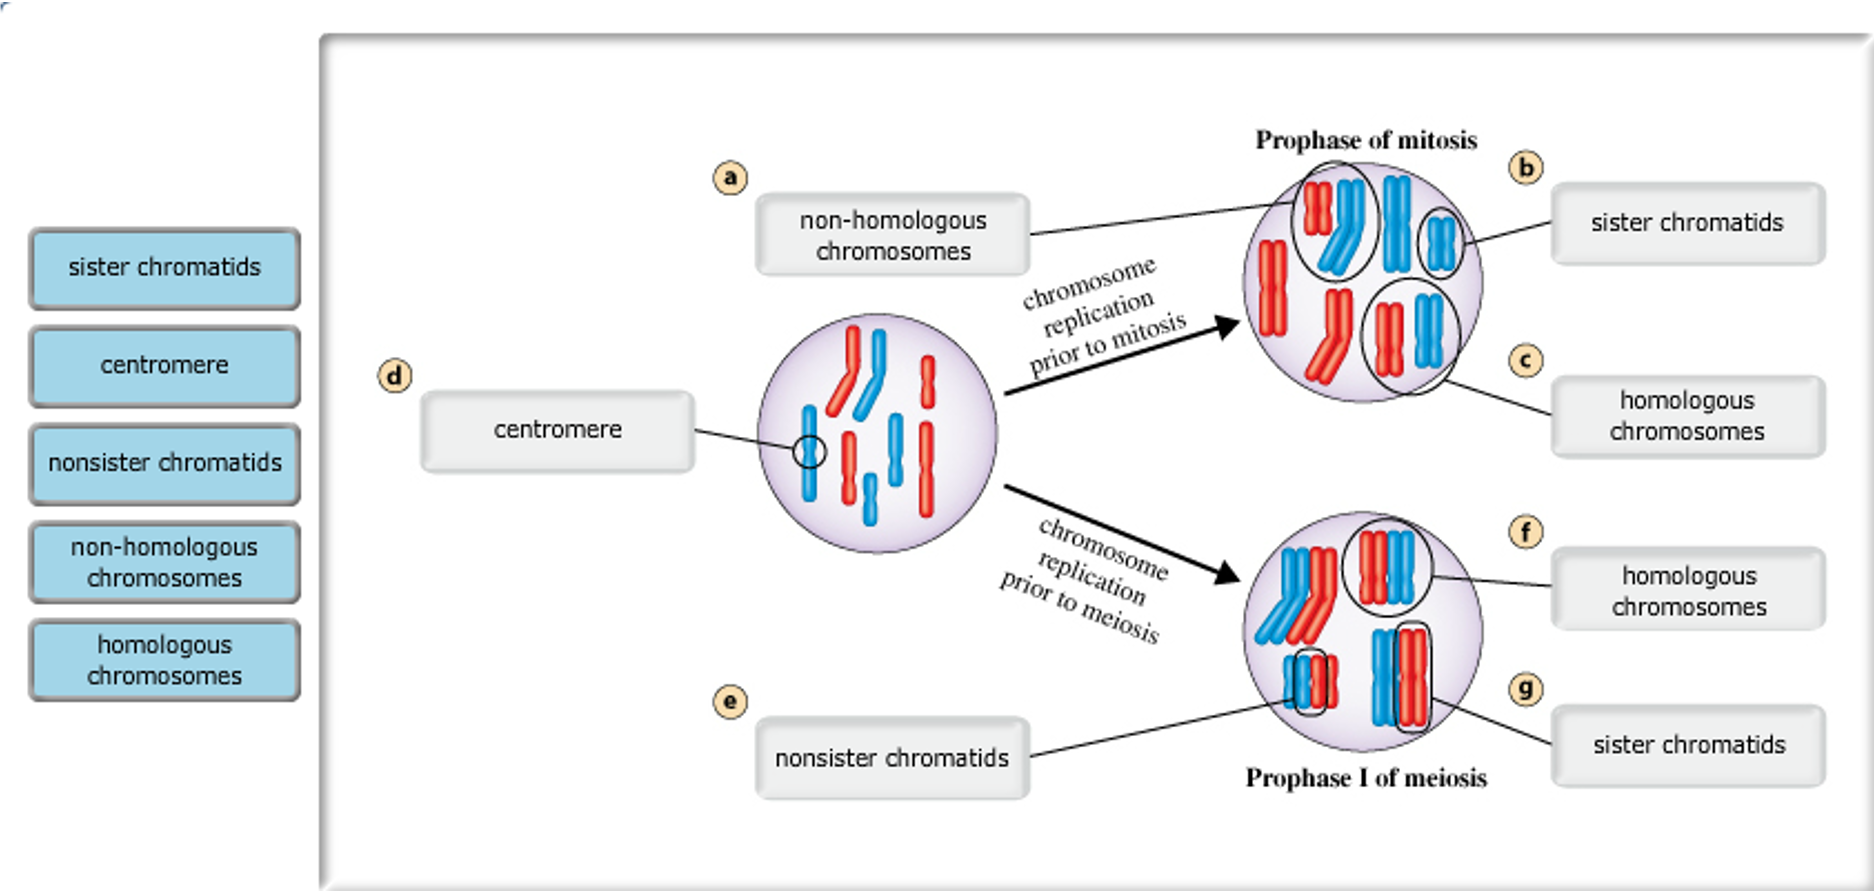
\includegraphics{./img/nonsis.png}

\textbf{D. The Phases of Meiosis}\\
1. Meiosis involves two divisions of the nucleus and the {cytoplasm}. These divisions, known as meiosis I and meiosis II, result in four haploid cells.\\
2. During {interphase}, the reproductive cell grows and duplicates its chromosomes.\\
3. During meiosis I, each pair of duplicated homologous chromosomes {separates}.\\
4. After meiosis I, the two cells formed during this stage go through a second division of the {nucleus} and cytoplasm called meiosis II. During meiosis II, sister {chromatids} separate to produce four haploid cells.

\textbf{E. Why is meiosis important?}\\
1. Meiosis forms sex cells with the correct haploid number of {chromosomes}. This maintains the correct {diploid} number of chromosomes in organisms when sex cells join. Meiosis creates genetic variation by producing {haploid} cells.

\hypertarget{homework-1}{%
\subsection{Homework}\label{homework-1}}

\textbf{Fill in the Blanks}\\
1. diploid; haploid\\
2. haploid; diploid\\
3. diploid\\
4. homologous chromosomes\\
5. homologous chromosomes\\
6. N/A\\
7. meiosis\\
8. sister chromatids\\
9. sister chromatids\\
10. meiosis; meiosis\\
11. meiosis

\textbf{Short Answer Questions}\\
12. Sex cells are haploid cells.

\hypertarget{lecture-6-meiosis-2}{%
\section{Lecture 6: Meiosis-2}\label{lecture-6-meiosis-2}}

\hypertarget{lesson-outline-2}{%
\subsection{Lesson outline}\label{lesson-outline-2}}

\begin{longtable}[]{@{}c@{}}
\toprule\noalign{}
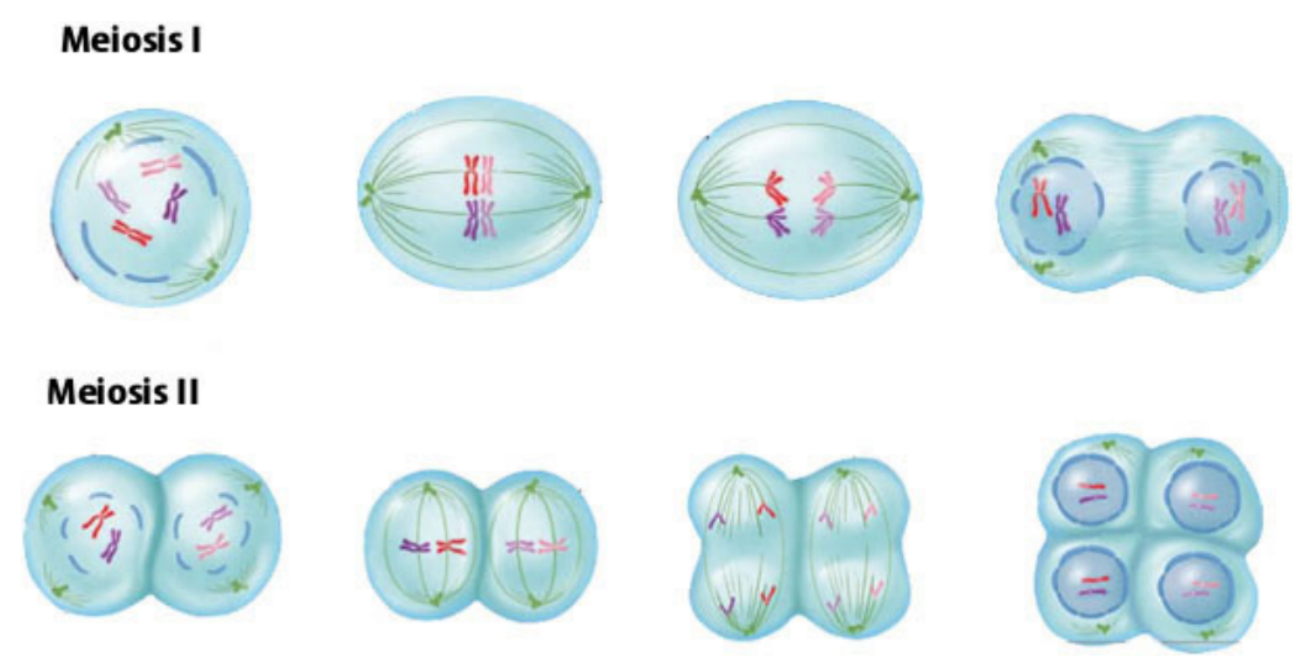
\includegraphics{./img/meiosis2.png} \\
\midrule\noalign{}
\endhead
\bottomrule\noalign{}
\endlastfoot
\emph{meiosis illustration 1} \\
\end{longtable}

\begin{longtable}[]{@{}c@{}}
\toprule\noalign{}
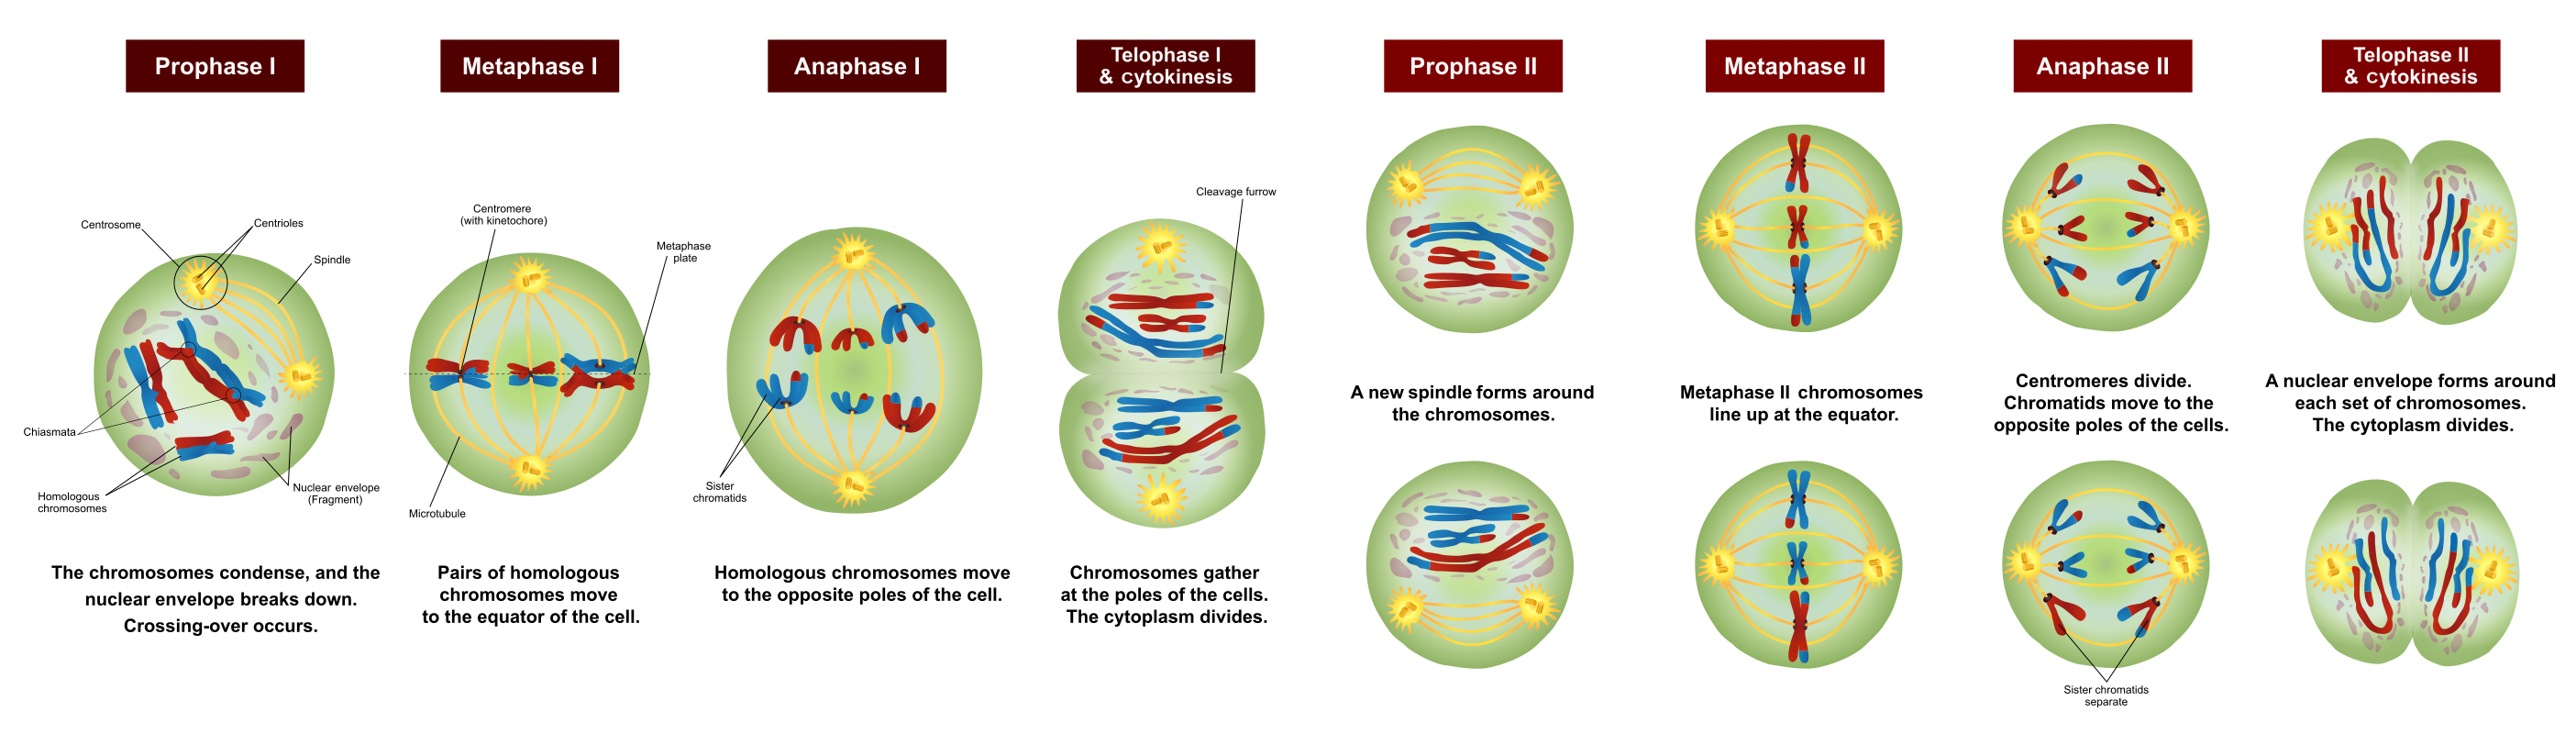
\includegraphics{./img/Meiosis_Stages.svg.png} \\
\midrule\noalign{}
\endhead
\bottomrule\noalign{}
\endlastfoot
\emph{meiosis illustration 2} \\
\end{longtable}

\begin{longtable}[]{@{}c@{}}
\toprule\noalign{}
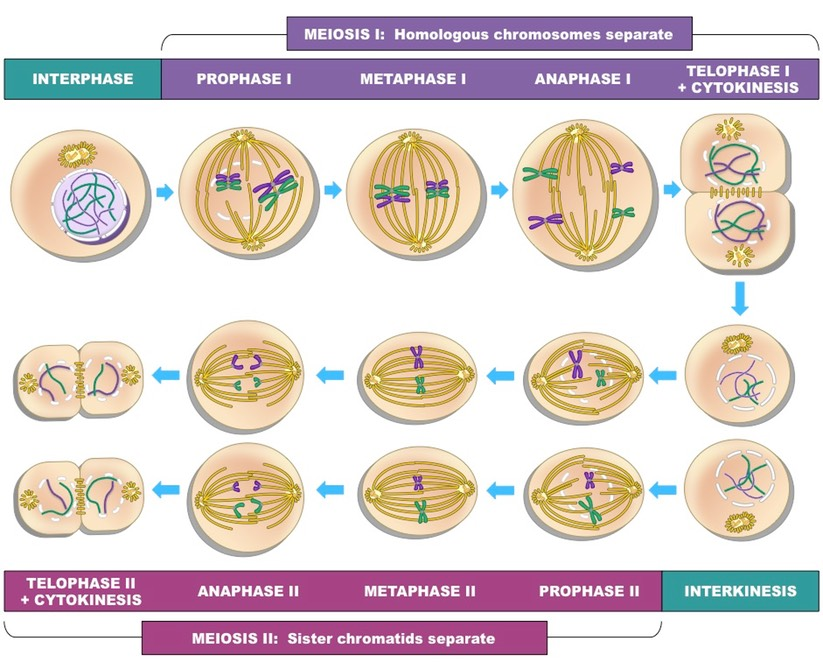
\includegraphics{./img/meiosis-complex_med.jpeg} \\
\midrule\noalign{}
\endhead
\bottomrule\noalign{}
\endlastfoot
\emph{meiosis illustration 3} \\
\end{longtable}

\begin{enumerate}
\def\labelenumi{\arabic{enumi}.}
\tightlist
\item
  interphase\\
\item
  Homologous chromosomes\\
\item
  breaks\\
\item
  middle\\
\item
  Spindle\\
\item
  homologous\\
\item
  Sister chromatids\\
\item
  two\\
\item
  Sister chromatids\\
\item
  Chromosomes; Nuclear membrane\\
\item
  align\\
\item
  pulled apart; opposite ends of the cells\\
\item
  chromosomes\\
\item
  four\\
\item
  half
\end{enumerate}

\hypertarget{homework-2}{%
\subsection{Homework}\label{homework-2}}

\textbf{Multiple Choice Questions}\\
1. A\\
2. C\\
3. C\\
4. D

\textbf{Short Answer Questions}\\
(6 points maximum) One point for each of the following:

\begin{itemize}
\item
  Correct description of meiosis\\
  Germ cell is a diploid cell, and goes through meiosis to produce gametes, which are haploid cells.\\
\item
  DNA replicates in interphase\\
  DNA replicates in interphase, and each chromosome then has a pair of identical sister chromatids.\\
\item
  Homologous chromosomes pair in prophase I\\
\item
  Spindle fibers move chromosomes pairs to poles in anaphase I\\
  In the end of meiosis I, two daughter cells are produced, and their chromosomes are halved.
\item
  Two cycles/rounds of division in meiosis\\
\item
  No additional replication before meiosis II\\
\item
  Sister chromatids separate to poles in anaphase II\\
  Separation of sister chromatids doesn't change the number of chromsomes. The daughter cells are still haploid cells.
\item
  1 germ cell yields 4 gametes\\
  4 gametes, which are haploid cells, are produced in the end of meiosis.
\end{itemize}

\textbf{Fill in the Blanks}\\
1. Anaphase II\\
2. N/A\\
3. Metaphase I\\
4. Telophase II (not quite obvious)\\
5. Telophase I (not quite obvious)\\
6. N/A\\
7. Metaphase II\\
8. Prophase I\\
9. Prophase II\\
10. Anaphase I

\hypertarget{lecture-7-meiosis-3}{%
\section{Lecture 7: Meiosis-3}\label{lecture-7-meiosis-3}}

\hypertarget{lesson-outline-3}{%
\subsection{Lesson outline}\label{lesson-outline-3}}

\textbf{F. How do mitosis and meiosis differ?}\\
1. During {mitosis} and cell division, a body cell and its nucleus divide once and produce two identical cells.\\
2. During {meiosis}, a reproductive cell and its nucleus divide twice and produce four cells----two pairs of identical haploid cells.

\textbf{G. Advantages of Sexual Reproduction}\\
1. Sexual reproduction produces {offspring} that have a new combination of DNA. This results in genetic {variation} among individuals.\\
2. Genetic variation gives individuals within a population slight differences that might be an advantage if the {environment} changes.\\
3. {Selective breeding} has been used to develop desirable traits in plants and animals.

\textbf{H. Disadvantages of Sexual Reproduction}\\
1. One disadvantage of sexual reproduction is that organisms have to grow and develop until they are mature enough to produce {sex} cells.\\
2. Another disadvantage is that searching for a mate takes time and energy and might expose individuals to predators, {diseases}, or harsh environmental conditions.

Compare and contrast meiosis and mitosis and cell division
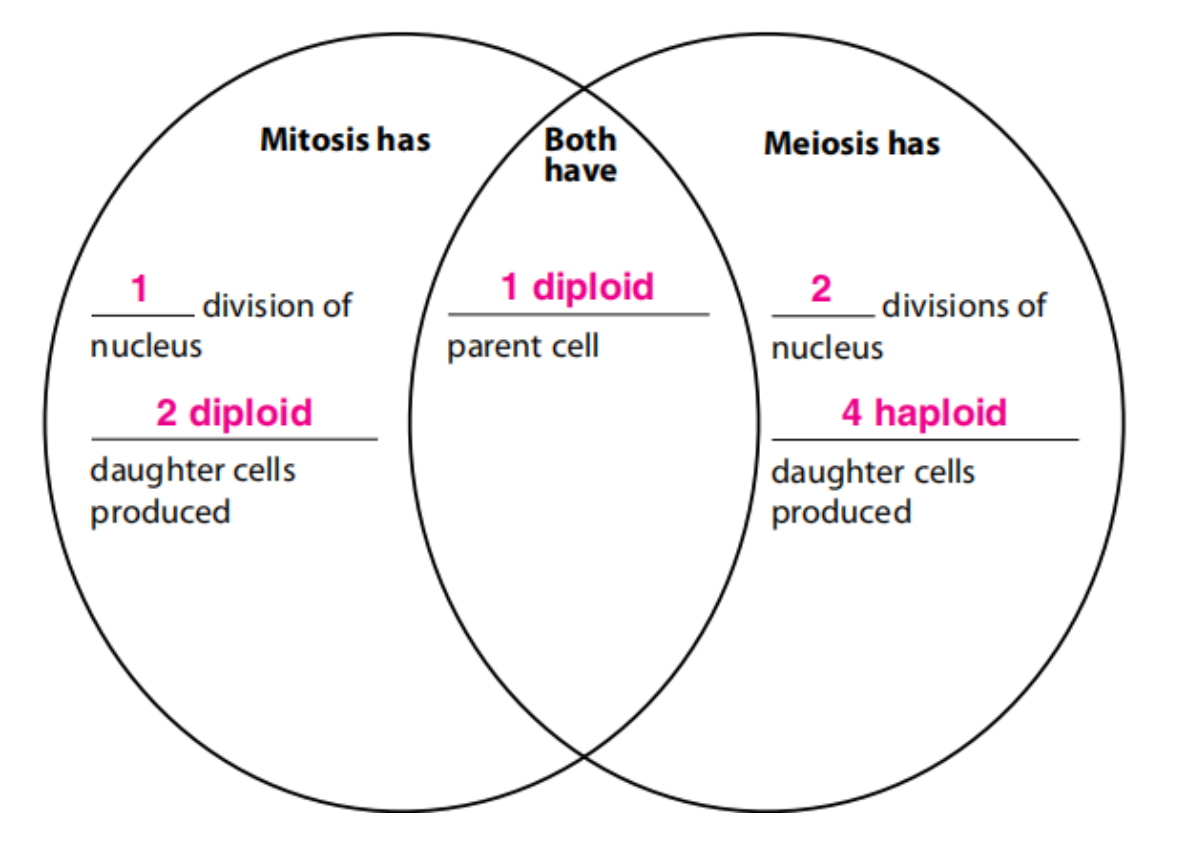
\includegraphics{./img/mitosis-meiosis.png}

\textbf{Explain} why genetic variation and selective breeding are advantages of sexual reproduction.\\
\textbf{Genetic variation}: Instead of being exact genetic copies of parents, members of the same species have different traits, which enable some of them to survive environmental changes.\\
\textbf{Selective breeding}: The process of choosing and breeding individuals with desirable traits allows breeders to create offspring with those traits.

\textbf{Identify} two main disadvantages of sexual reproduction.\\
1. takes time and takes energy\\
2. sexual reproduction is limited by certain factors (For example, fertilization cannot take place during pregnancy, which can last as long as two years in some mammals.)

\textbf{Explain} how the process of meiosis relates to the way in which a child resembles but is not an exact copy of his or her parents.\\
Observable characteristics in a child, such as \textbf{eye color, hair type and color, the shapes of facial features, and height}, resemble those of his or her parents, because the child \textbf{inherits portions of DNA from each parent}. A child is not a exact copy of his or her parents because the child \textbf{does not carry identical DNA to either parent}.

\hypertarget{homework-3}{%
\subsection{Homework}\label{homework-3}}

\textbf{Multiple Choice Questions}\\
1. D\\
2. C\\
(Hint: Crossing over)

\textbf{Short Answer Questions}

\begin{itemize}
\tightlist
\item
  Organism: correct organism that produces sexually\\
\item
  Mode: two different parents / egg and sperm combine in fertilization / gametes (1n) combine to form zygote (2n) / fertilization is random\\
\item
  Advantage: increase genetic variations
\end{itemize}

\textbf{Enrichment}\\
1. For many generations, {native plants that were resistant to disease and pests} survived and reproduced. The resistant traits were passed on to their offspring. Meanwhile, {those native plants that were not resistant to disease and pests} died off. Eventually, the population of native plants was made up mainly of resistant plants.\\
2. Possible answers:\\
Preserve all: Many plants that have no current known value might have important uses in the future. Saving plants that aren't useful to people is still necessary because other organisms might depend upon these plants for survival.\\
Preserve some: Because of budget restrictions, some plants might be targeted for preservation and others are allowed to become extinct. In this situation, it would be best to determine which plants are likely to be useful to people.

\hypertarget{lecture-8-asexual-reproduction}{%
\section{Lecture 8: Asexual Reproduction}\label{lecture-8-asexual-reproduction}}

\hypertarget{keywords-1}{%
\subsection{Keywords}\label{keywords-1}}

\begin{longtable}[]{@{}cc@{}}
\toprule\noalign{}
英文 & 中文 \\
\midrule\noalign{}
\endhead
\bottomrule\noalign{}
\endlastfoot
Asexual reproduction & 无性生殖 \\
Fission & 裂殖 \\
Budding & 出芽生殖 \\
Regeneration & 再生 \\
vegetative reproduction & 营养器官繁殖 \\
Culture medium & 培养基 \\
Potential & 潜能 \\
Cloning & 克隆 \\
\end{longtable}

\hypertarget{lesson-outline-4}{%
\subsection{Lesson outline}\label{lesson-outline-4}}

\textbf{A. What is asexual reproduction?}\\
1. In {asexual reproduction}, one parent organism produces offspring without meiosis and fertilization.\\
2. Because the offspring of asexual reproduction inherit all their DNA from one parent, they are genetically {identical} to each other and their parent.

\textbf{B. Types of Asexual Reproduction}\\
1. Cell division in prokaryotes is known as {\textbf{fission}}.\\
2. During fission, DNA is {copied} and the cell splits to form two identical offspring. The original cell no longer exists.\\
3. Many unicellular {eukaryotes} reproduce by {\textbf{mitotic cell division}}. In this type of asexual reproduction, an organism forms two offspring through mitosis and {cell division}.\\
4. In {\textbf{budding}}, a new organism grows on the body of its parent by mitosis and cell division. When the bud becomes large enough, it can break from the parent and live on its own.\\
5. {\textbf{Regeneration}} occurs when an offspring grows from a piece of its parent.\\
a. Sea stars, sea urchins, sea cucumbers, and planarians can {reproduce} through regeneration.\\
b. Many animals can {regenerate} damaged or lost body parts. This is not reproduction; {new individuals} are not produced.\\
6. {\textbf{Vegetative reproduction}} is a form of asexual reproduction in which offspring grow from a part of a parent plant.\\
7. {\textbf{Cloning}} is a type of asexual reproduction developed by scientists and performed in laboratories. It produces {identical} individuals from a cell or from a cluster of cells taken from a multicellular organism.\\
8. Using a cloning method called {tissue culture}, plant growers and scientists use a meristem to make a copy of a plant with desirable traits.\\
9. Because all of a clone's {chromosomes} come from one parent, the clone is a genetic copy of its parent.\\
10. Asexual reproduction enables organisms to reproduce without a(n) {mate}.\\
11. Asexual reproduction also enables some organisms to rapidly produce a large number of {offspring}.\\
12. Asexual reproduction produces offspring that are genetically identical to each other and to their parent. This results in little genetic {variation} within a population.\\
13. Genetic variation is important because it can increase an organism's chance of {surviving} if the environment changes.\\
14. Genetic changes, called {mutations}, can occur and then be passed to offspring; this can affect the offspring's ability to survive.

\hypertarget{homework-4}{%
\subsection{Homework}\label{homework-4}}

\textbf{Matching}\\
1.B\\
2.A\\
3.C\\
4.D\\
5.F\\
6.E

\textbf{Multiple Choice Questions}\\
7.D\\
8.B\\
9.C\\
10.C\\
11.C\\
12.C\\
13.B\\
14.B

\textbf{Enrichment}\\
1. The extreme cold that preserved the woolly mammoths also damaged their cells.
Scientists need whole cells to clone an animal.\\
2. Possible answer: Scientists might be able to understand why the animal became
extinct. They might also learn more about the animal's physical characteristics and its behaviors, as well as its environment.

\hypertarget{midterm-review}{%
\chapter{Midterm Review}\label{midterm-review}}

\hypertarget{midterm-review-scope}{%
\section{Midterm Review Scope}\label{midterm-review-scope}}

\hypertarget{midterm-review-practice-1}{%
\section{Midterm Review Practice 1}\label{midterm-review-practice-1}}

\hypertarget{midterm-review-practice-2}{%
\section{Midterm Review Practice 2}\label{midterm-review-practice-2}}

\hypertarget{chapter-iii-genetics}{%
\chapter{Chapter III: Genetics}\label{chapter-iii-genetics}}

\includegraphics{./img/ch3.png}

\hypertarget{lecture-9-mendel-and-his-peas---1}{%
\section{Lecture 9: Mendel and his Peas - 1}\label{lecture-9-mendel-and-his-peas---1}}

\hypertarget{keywords-2}{%
\subsection{Keywords}\label{keywords-2}}

\begin{longtable}[]{@{}
  >{\centering\arraybackslash}p{(\columnwidth - 4\tabcolsep) * \real{0.2742}}
  >{\centering\arraybackslash}p{(\columnwidth - 4\tabcolsep) * \real{0.1935}}
  >{\centering\arraybackslash}p{(\columnwidth - 4\tabcolsep) * \real{0.5323}}@{}}
\toprule\noalign{}
\begin{minipage}[b]{\linewidth}\centering
英文
\end{minipage} & \begin{minipage}[b]{\linewidth}\centering
中文
\end{minipage} & \begin{minipage}[b]{\linewidth}\centering
解释
\end{minipage} \\
\midrule\noalign{}
\endhead
\bottomrule\noalign{}
\endlastfoot
Trait & 性状 & characteristic \\
Heredity & 遗传 & the passing of traits from parents to offspring \\
Genetics & 遗传学 & the study of how traits are passed on \\
Self-pollination & 自花授粉 & a form of pollination when pollen from one plant lands on the pistil of a flower on the same plant \\
Cross-pollination & 异花授粉 & a form of pollination when pollen from one plant reaches the pistil of a flower on a different plant \\
Pistil & 雌蕊 & female organs of a flower \\
Stigma & 柱头 & the part of a pistil that receives the pollen during pollination \\
Stamen & 雄蕊 & male organs of a flower \\
Anther & 花药 & the part of a stamen that contains the pollen \\
Pollen & 花粉 & consists of pollen grains, which produce male gametes (sperm cells) \\
True-breeding & 纯种 & organisms whose offspring are the same as the parent \\
Hybrid & 杂种 & organisms from true-breeding parents with different traits \\
\end{longtable}

\hypertarget{lesson-outline-5}{%
\subsection{Lesson outline}\label{lesson-outline-5}}

\textbf{A. Early Ideas about Heredity}\\
1. {Heredity} is the passing of traits from parents to offspring.\\
2. In the 1850s, {Gregor Mendel}, an Austrian monk, performed experiments that helped answer questions about how traits are inherited.\\
3. {Genetics} is the study of how traits pass from parents to offspring.

\textbf{B. Mendel's Experimental Methods}\\
1. Pea plants were ideal for genetic studies because they {reproduce} quickly; they have easily observed {traits}; and the experimenter can control which pairs of plants {reproduce}.\\
2. Mendel controlled which plants {pollinated} other plants.\\
    a. When a(n) {true-breeding} plant self-pollinates, it always produces offspring with traits that match the parent.\\
    b. By {cross-pollinating} plants himself, Mendel was able to select which plants pollinated other plants.\\
3. With each cross-pollination Mendel did, he recorded the traits that appeared in the {offspring}.

\textbf{C. Mendel's Results}\\
1. Mendel's crosses between true-breeding plants with purple flowers produced plants with only {purple} flowers. Crosses between true-breeding plants with white flowers produced plants with only {white} flowers.\\
2. Crosses between true-breeding plants with purple flowers and true-breeding plants with white flowers produced plants with only {purple} flowers.\\
3. The first--generation purple-flowering plants are called {hybrid} plants.\\
4. When Mendel cross-pollinated two hybrid plants, the trait that had disappeared in the first generation always {reappeared} in the second generation.\\
5. Mendel analyzed the data from many experiments on seven different {traits}. He always noted a 3:1 {ratio}; for example, purple flowers grew from hybrid crosses {three} times as often as white flowers.

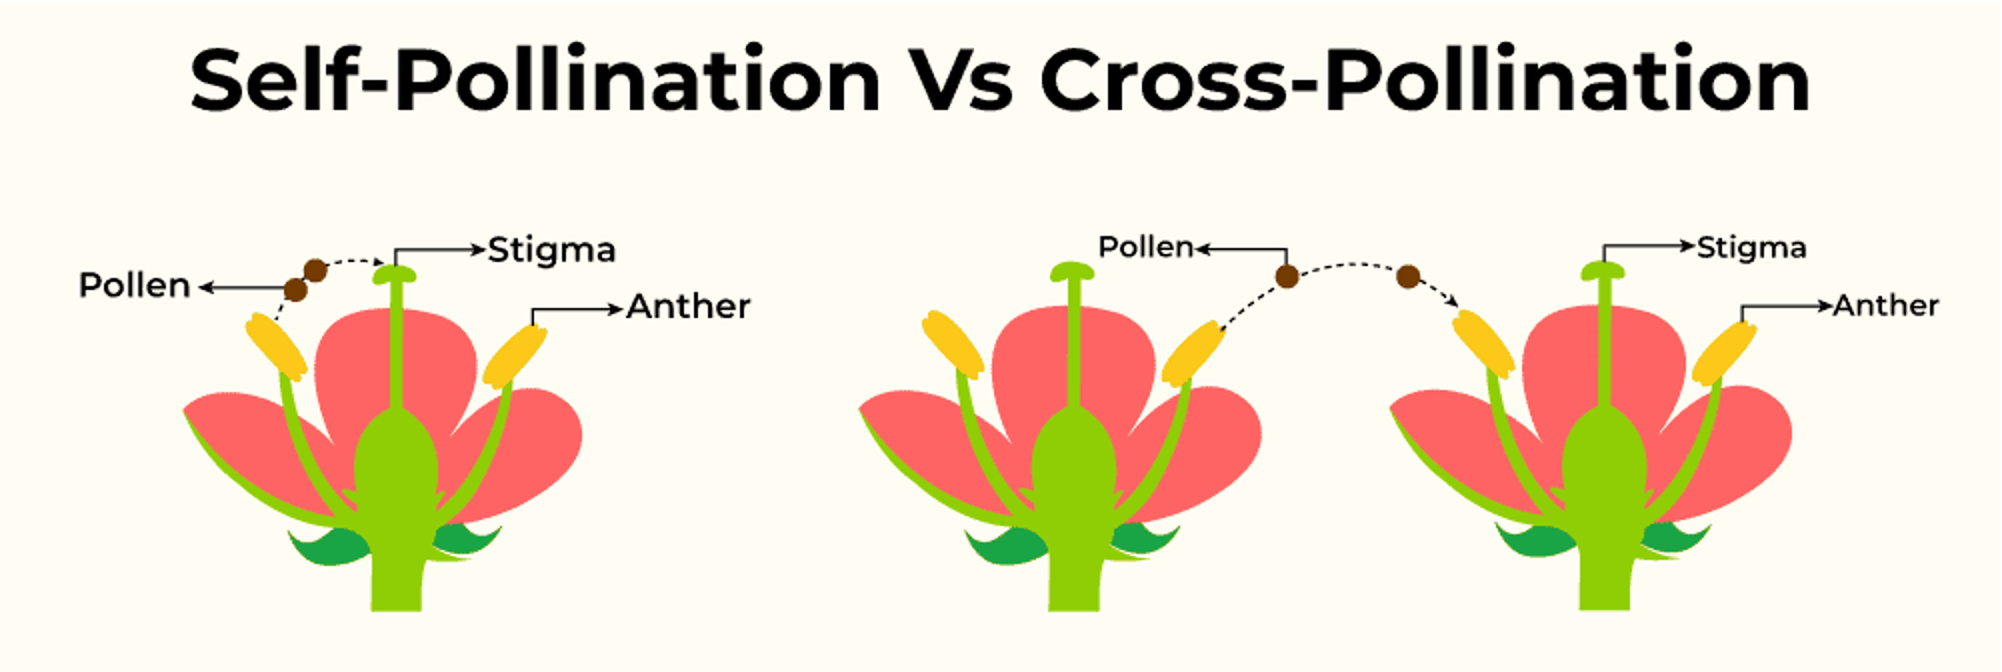
\includegraphics{./img/l9-1.png}

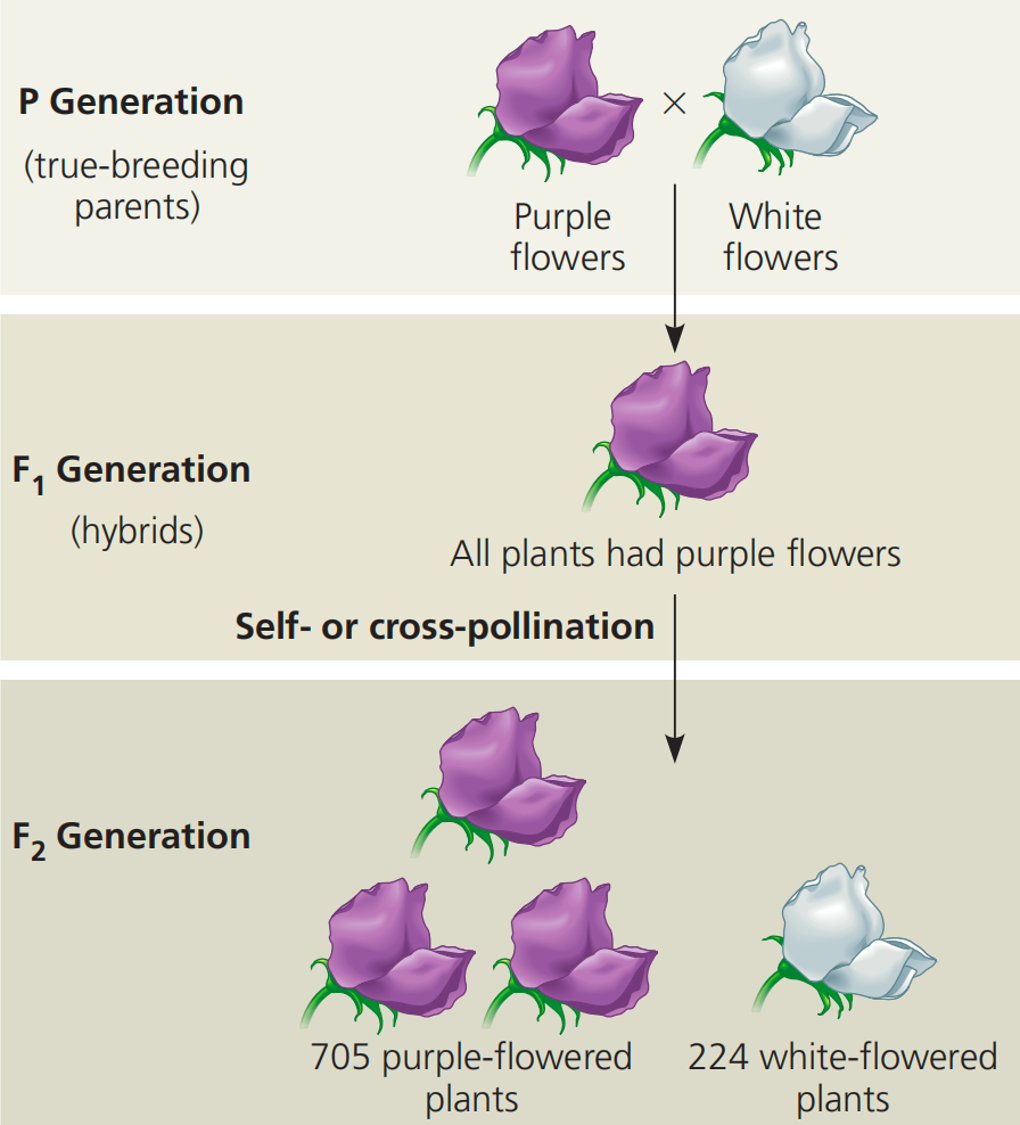
\includegraphics{./img/l9-2.png}

  \bibliography{book.bib,packages.bib}

\end{document}
